%-----------------------------------------------------------------------------%
\chapter{\babLima}
%-----------------------------------------------------------------------------%

%-----------------------------------------------------------------------------%
\section{Perubahan pada Struktur Zotonic}
%-----------------------------------------------------------------------------%

Agar ontologi dan \textit{web services} dapat terintegrasi, terdapat beberapa berkas baru yang ditambahkan ke dalam struktur Zotonic. Berikut adalah struktur dari Zotonic yang telah dapat membuat struktur Zotonic dari ontologi sebelum penambahan berkas baru untuk menjalankan fungsi integrasi ontologi dan \textit{web service}\\
	\begin{tabbing}
		\qquad Zotonic/ \\
		\qquad \qquad .rebar/ \\
		\qquad \qquad bin/ \\
		\qquad \qquad deps/ \\
		\qquad \qquad doc/ \\
		\qquad \qquad docker/ \\
		\qquad \qquad ebin/ \\
		\qquad \qquad include/ \\
		\qquad \qquad modules/ \\
		\qquad \qquad priv/ \\
		\qquad \qquad src/ \\
		\qquad \qquad user/ \\
		\qquad \qquad .dockerignore \\
		\qquad \qquad .editorconfig \\
		\qquad \qquad .travis.yml \\
		\qquad \qquad AUTHORS \\
		\qquad \qquad CONTRIBUTING.md \\
		\qquad \qquad CONTRIBUTORS \\
		\qquad \qquad Dockerfile \\
		\qquad \qquad Dockerfile.dev \\
		\qquad \qquad Dockerfile.heavy \\
		\qquad \qquad GNUmakefile \\
		\qquad \qquad LICENSE\\
		\qquad \qquad Makefile \\
		\qquad \qquad Readme.md \\
		\qquad \qquad TRANSLATORS \\
		\qquad \qquad USE\_REBAR\_LOCKED \\
		\qquad \qquad build.cmd \\
		\qquad \qquad charity\_org\_rdf.owl \\
		\qquad \qquad classAndObjectPropertyMapper.sh \\
		\qquad \qquad docker-compose.yml \\
		\qquad \qquad prepare-release.sh \\
		\qquad \qquad rebar \\
		\qquad \qquad rebar.config\\
		\qquad \qquad rebar.config.lock\\
		\qquad \qquad rebar.config.lock.script\\
		\qquad \qquad rebar.config.script\\
		\qquad \qquad recentsite.txt\\
		\qquad \qquad start.cmd\\
		\qquad \qquad start.sh\\
		\qquad \qquad zotonic.pid\\
		\qquad \qquad zotonic\_install
	\end{tabbing}
	
	Setelah implementasi, perlu ditambahkan berkas rules.txt pada folder Zotonic dimana berkas ini merupakan tabel \textit{rules} yang akan digunakan untuk \textit{mapping web service} seperti yang dijelaskan pada bab sebelumnya. Selain itu, perlu ditambahkan juga modul m\_abs.erl pada folder \textit{models} yang terdapat pada folder \textit{src} dari folder Zotonic. Modul ini yang nantinya akan berfungsi sebagai \textit{adaptor} untuk menghubungkan antara ontologi dan \textit{web services} seperti penjelasan pada bab sebelumnya.
		
%-----------------------------------------------------------------------------%
\section{Perubahan Setelah \textit{Create Site Script} Dijalankan}
%-----------------------------------------------------------------------------%

Setelah menjalankan proses \textit{build script}, maka \textit{site} dapat dibuat dengan menjalankan proses \textit{create site script}. Langkah untuk menjalankan \textit{create site script} sebagai berikut

\begin{enumerate}
	\item Jalankan Zotonic dengan perintah seperti kode \ref{lst:debug} untuk menjalankan Zotonic dalam mode debug atau \ref{lst:startzotonic} untuk menjalankan Zotonic tanpa debug.
	
	\begin{minipage}{\linewidth}
		\begin{lstlisting}[caption={Perintah untuk menjalankan Zotonic pada mode \textit{debug}},label={lst:debug}]
		$ bin/zotonic debug
		\end{lstlisting}
	\end{minipage}

	\begin{minipage}{\linewidth}
		\begin{lstlisting}[caption={Perintah untuk menjalankan Zotonic tanpa mode \textit{debug}},label={lst:startzotonic}]
		$ bin/zotonic start
		\end{lstlisting}
	\end{minipage}

	\item Persiapkan database pgsql untuk \textit{site} yang akan dibuat dengan membuat \textit{user} baru bernama Zotonic dengan \textit{password} Zotonic pada pgsql. Lalu beri akses kepada \textit{user} tersebut untuk dapat membuat database baru.
	
	\item Setelah mempersiapkan database, selanjutnya edit berkas \co{/etc/hosts} dengan menambahkan namasite.dev yang diarahkan menuju local host seperti pada kode \ref{lst:etchosts}. namasite merupakan nama dari \textit{site} yang ingin dibuat. Dalam penelitian ini, penulis membuat site bsmi sehingga namasite akan diubah menjadi bsmi
	\begin{minipage}{\linewidth}
		\begin{lstlisting}[caption={Configurasi berkas /etc/hosts},label={lst:etchosts}]
		127.0.0.1   namasite.dev
		\end{lstlisting}
	\end{minipage}

	\item Selanjutnya dapat menjalankan perintah seperti kode \ref{lst:createsite}, untuk membuat \textit{site} baru pada Zotonic dengan \textit{template} blog
	\begin{minipage}{\linewidth}
		\begin{lstlisting}[caption={Perintah untuk membuat \textit{site} baru pada Zotonic},label={lst:createsite}]
		$ bin/zotonic addsite -s blog namasite
		\end{lstlisting}
	\end{minipage}

	\item Setelah proses \textit{create site} selesai, berhentikan Zotonic dengan menekan \co{Ctrl + C} dua kali jika menggunakan mode debug, atau menggunakan perintah seperti kode \ref{lst:stopzotonic} jika menjalankan Zotonic tanpa mode debug
	\begin{minipage}{\linewidth}
		\begin{lstlisting}[caption={Perintah untuk memberhentikan Zotonic},label={lst:stopzotonic}]
		$ bin/zotonic stop
		\end{lstlisting}
	\end{minipage}

	\item Selanjutnya jalankan perintah \co{make} untuk melakukan \textit{build} ulang pada Zotonic. Setelah selesai, jalankan lagi Zotonic seperti pada langkah 1
	
\end{enumerate}

Setelah proses diatas, Zotonic akan membuat sebuah folder baru pada \co{user/site/} dengan nama folder sesuai dengan namasite yang dibuat. Pada penelitian ini, folder tersebut bernama bsmi karena namasite yang digunakan adalah bsmi. Perubahan yang terjadi dapat dilihat pada berkas page.tpl yang terletak pada folder \textit{template} dari folder bsmi dimana untuk melakukan perhitungan \textit{business logic} sudah memanfaatkan \textit{adaptor} yang telah diimplementasikan pada bab sebelumnya.
\begin{minipage}{\linewidth}
	\begin{lstlisting}[caption={\textit{Business logic} untuk fungsi total pada kategori program},label={lst:totalfront}]
	...
	<p class="programtotal" id="programtotal">
		<b>{_ total _}</b> : 
	</p>
	 
		var total = {{m.abs.totalDonation[{query id=id}]}}; 
		if (total == 0) {
			document.getElementById("programtotal").className += " hidden"; } 
		else { 
			document.getElementById("programtotal").innerHTML += total;}
	
	...
	\end{lstlisting}
\end{minipage}

Pada kode \ref{lst:totalfront} dapat dilihat bahwa variabel total akan menerima nilai dari hasil pemanggilan \textit{adaptor} dengan fungsi \textit{totalDonation}. Dengan memanfaatkan \textit{adaptor}, akan mempermudah pengguna karena tidak perlu untuk melakukan implementasi \textit{business logic} pada kode program.
%-----------------------------------------------------------------------------%
\section{Contoh Penerapan pada Web BSMI}
%-----------------------------------------------------------------------------%

Setelah membuat \textit{site} baru pada Zotonic, tampilan awal dari \textit{site} tersebut seperti pada gambar \pic~\ref{fig:home}. Tampilan \textit{homepage} dari \textit{site} tersebut telah menggunakan \textit{bootstrap} sebagai css.
\begin{figure}
	\centering
	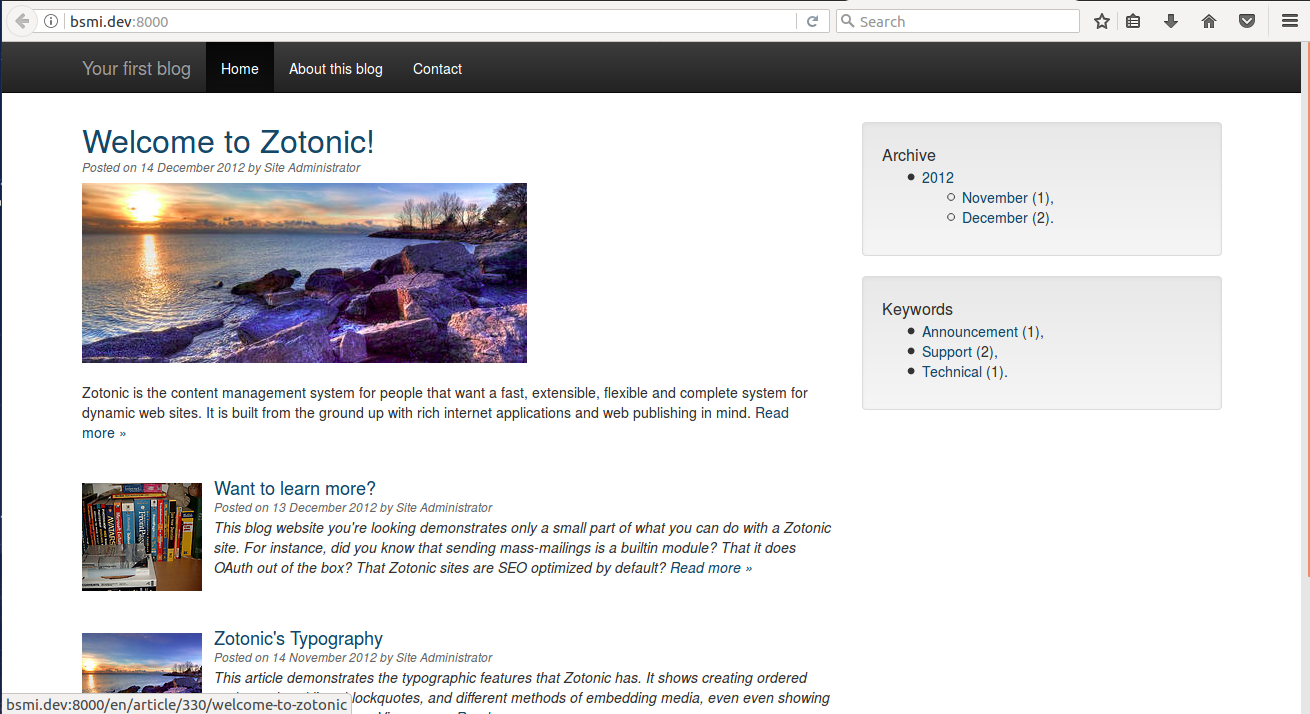
\includegraphics[width=1\textwidth]
	{pics/1-home.png}
	\caption{Tampilan awal \textit{site} pada Zotonic}
	\label{fig:home}
\end{figure}
\vspace{-0.3cm}

Selain \textit{homepage}, Zotonic sebagai sebuah CMS juga telah menyediakan halaman admin untuk pengguna agar dapat mengatur isi dari \textit{site} tersebut. Untuk dapat masuk ke dalam halaman admin, pengguna dapat mengakses halaman admin pada namasite.dev:8000/en/admin. Setelah mengakses halaman tersebut, pengguna akan melihat halaman untuk \textit{logon} seperti pada \pic~\ref{fig:logon}. Akun \textit{default} untuk \textit{logon} sebagai admin adalah \textit{username} admin dengan \textit{password} admin.
\begin{figure}
	\centering
	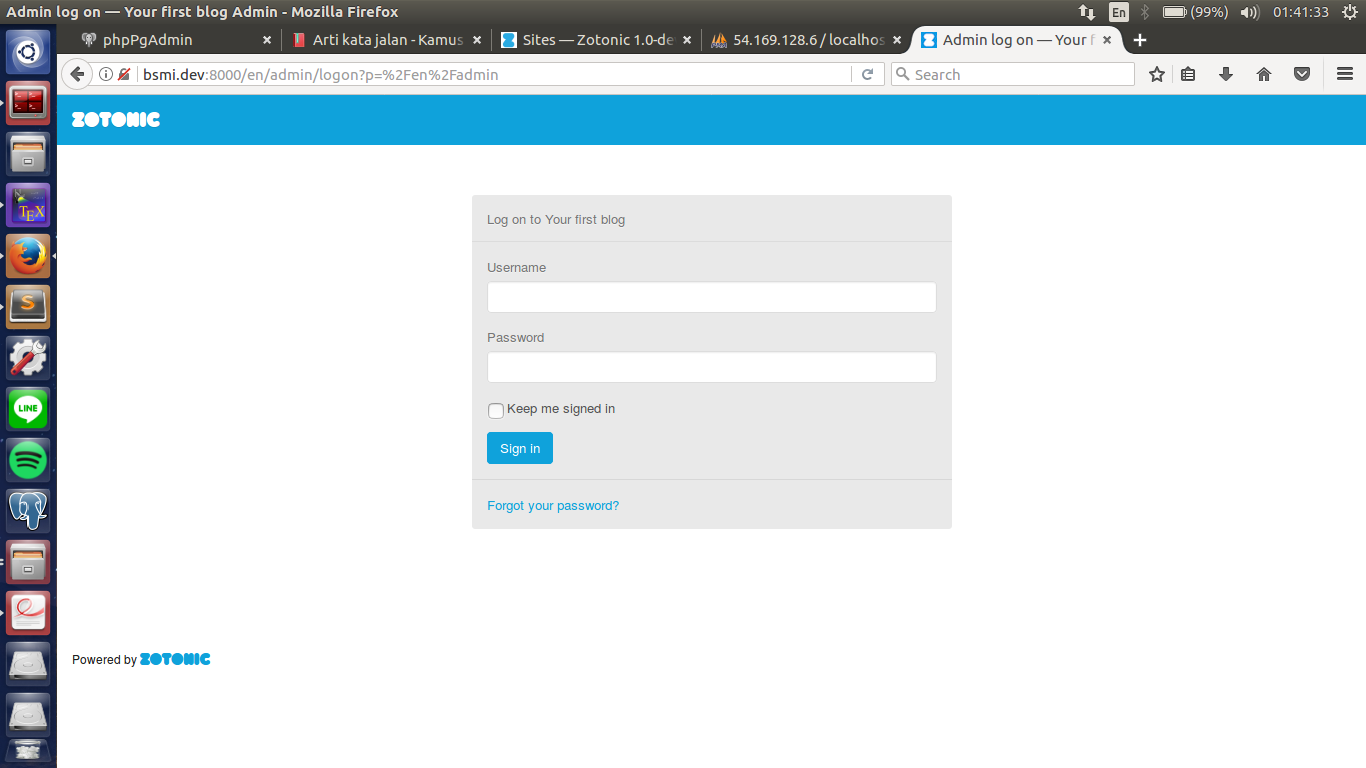
\includegraphics[width=1\textwidth]
	{pics/2-adminLogon.png}
	\caption{Tampilan login admin pada Zotonic}
	\label{fig:logon}
\end{figure}
\vspace{-0.3cm}

Setelah berhasil untuk \textit{logon}, pengguna akan melihat halaman \textit{dashboard} admin seperti pada \pic~\ref{fig:dashboard}. Pada \textit{dashboard} admin ini, sama seperti CMS lainnya dimana pengguna dapat melakukan berbagai hal seperti menambahkan konten dari \textit{site}, menambahkan \textit{user} baru untuk \textit{logon}, mengatur \textit{module-module} yang digunakan pada \textit{site}, dan lain-lain.
\begin{figure}
	\centering
	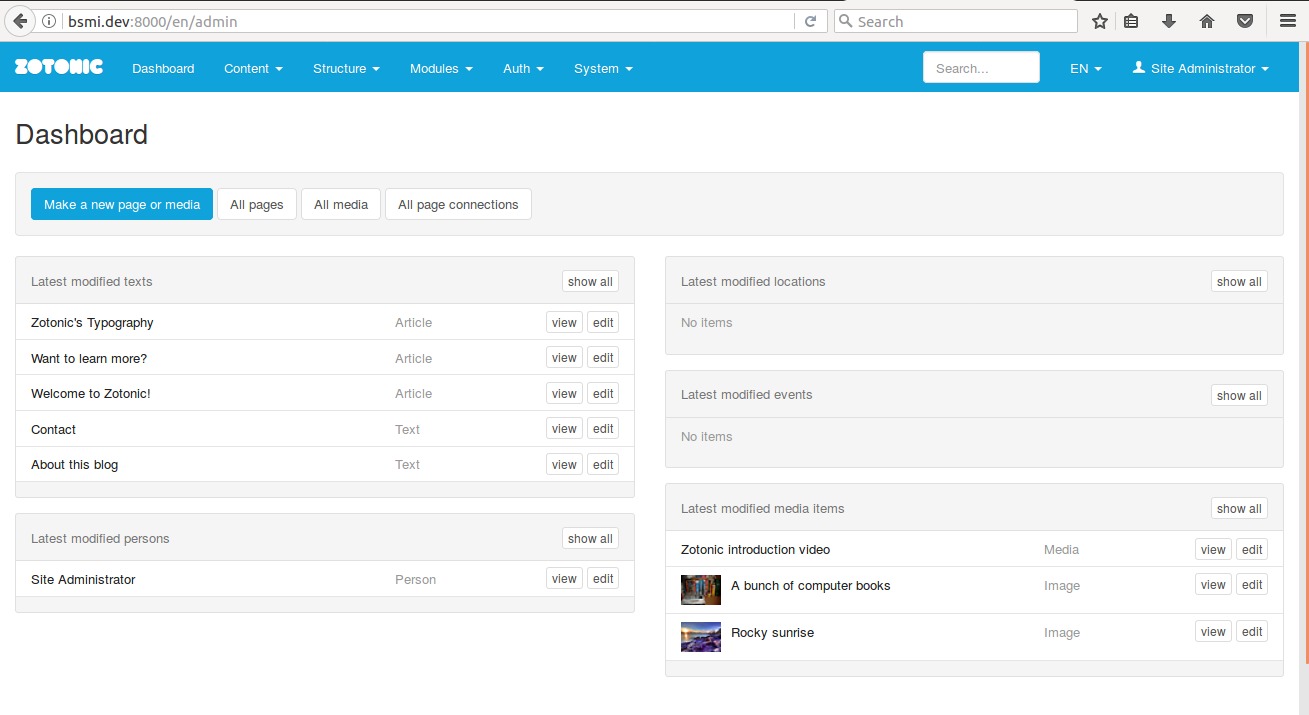
\includegraphics[width=1\textwidth]
	{pics/3-adminDashboard.png}
	\caption{Tampilan \textit{dashboard} admin pada Zotonic}
	\label{fig:dashboard}
\end{figure}
\vspace{-0.3cm}

Untuk dapat melihat apakah hasil implementasi pada bab sebelumnya sudah bekerja atau belum, maka perlu dibuat sebuah \textit{page} baru dengan kategori program pada \textit{site}. Hal ini dapat dilakukan dengan menekan tombol berwarna biru dengan tulisan \textit{Make a new page or media} pada \textit{dashboard} admin. Selanjutnya akan muncul \textit{modals} untuk membuat \textit{page} baru seperti pada gambar \pic~\ref{fig:createprogram}. Setelah mengisi nama dan memilih kategori program, \textit{checklist} pada \textit{published} agar \textit{page} dapat ditampilkan pada site. Selanjutnya klik tombol \textit{Make page}.

\begin{figure}
	\centering
	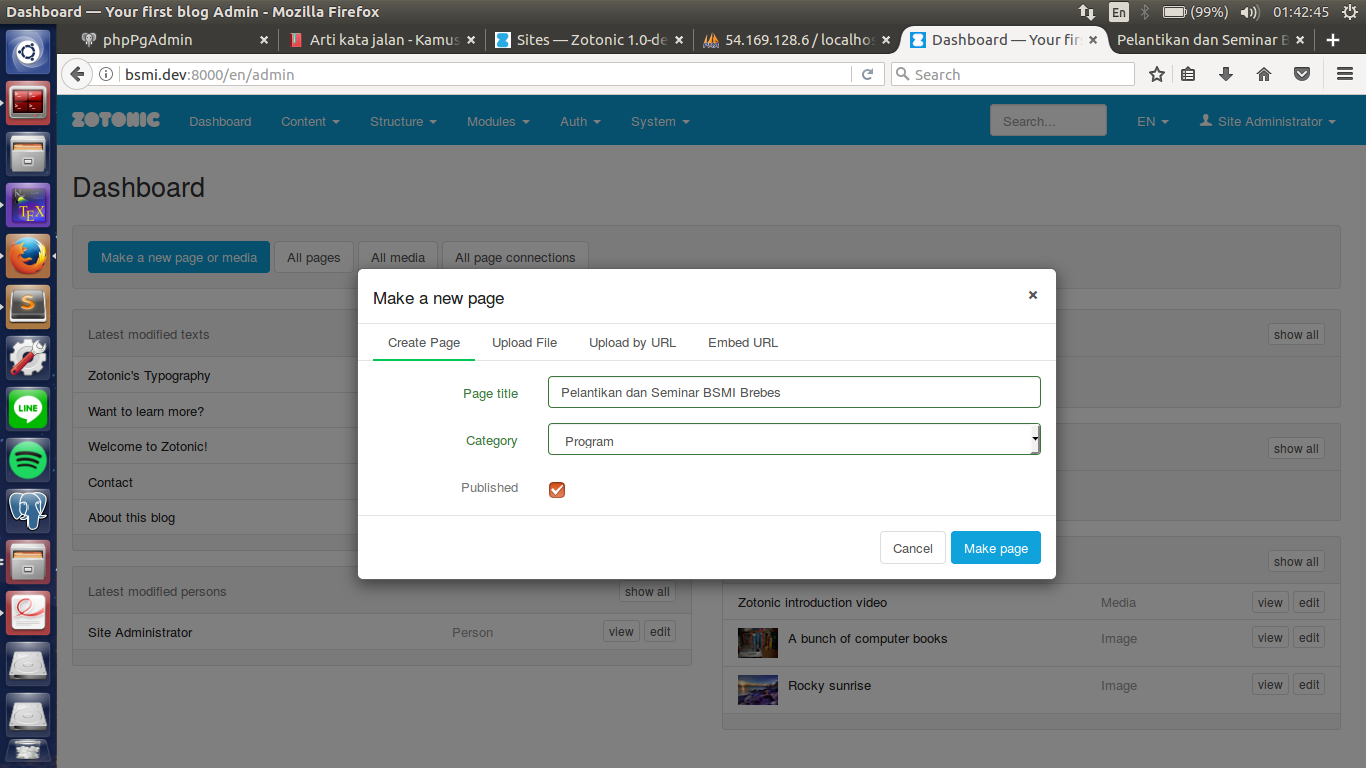
\includegraphics[width=1\textwidth]
	{pics/3-createProgram.png}
	\caption{Tampilan membuat \textit{page} pada Zotonic}
	\label{fig:createprogram}
\end{figure}
\vspace{-0.3cm}

Selanjutnya pengguna akan dibawa menuju sebuah halaman untuk mengubah detail dari \textit{page} yang dibuat seperti pada \pic~\ref{fig:editprogram}. Program memiliki sebuah \textit{data properties} yaitu total, dimana total akan diubah otomatis menggunakan \textit{business logic} berdasarkan donasi yang ada. Namun karena belum terdapat donasi yang terhubung pada program ini, sehingga nilai dari total bernilai 0. Pada halaman ini pengguna dapat menambahkan informasi seperti \textit{summary} dari \textit{page} yang dibuat atau menambahkan konten dari \textit{page} dan gambar seperti \pic~\ref{fig:editprogram2}. Selain itu, pada halaman ini pengguna juga dapat menambahkan \textit{page connection} agar halaman yang sedang dibuat dapat memiliki keterkaitan dengan halaman lainnya.
\begin{figure}
	\centering
	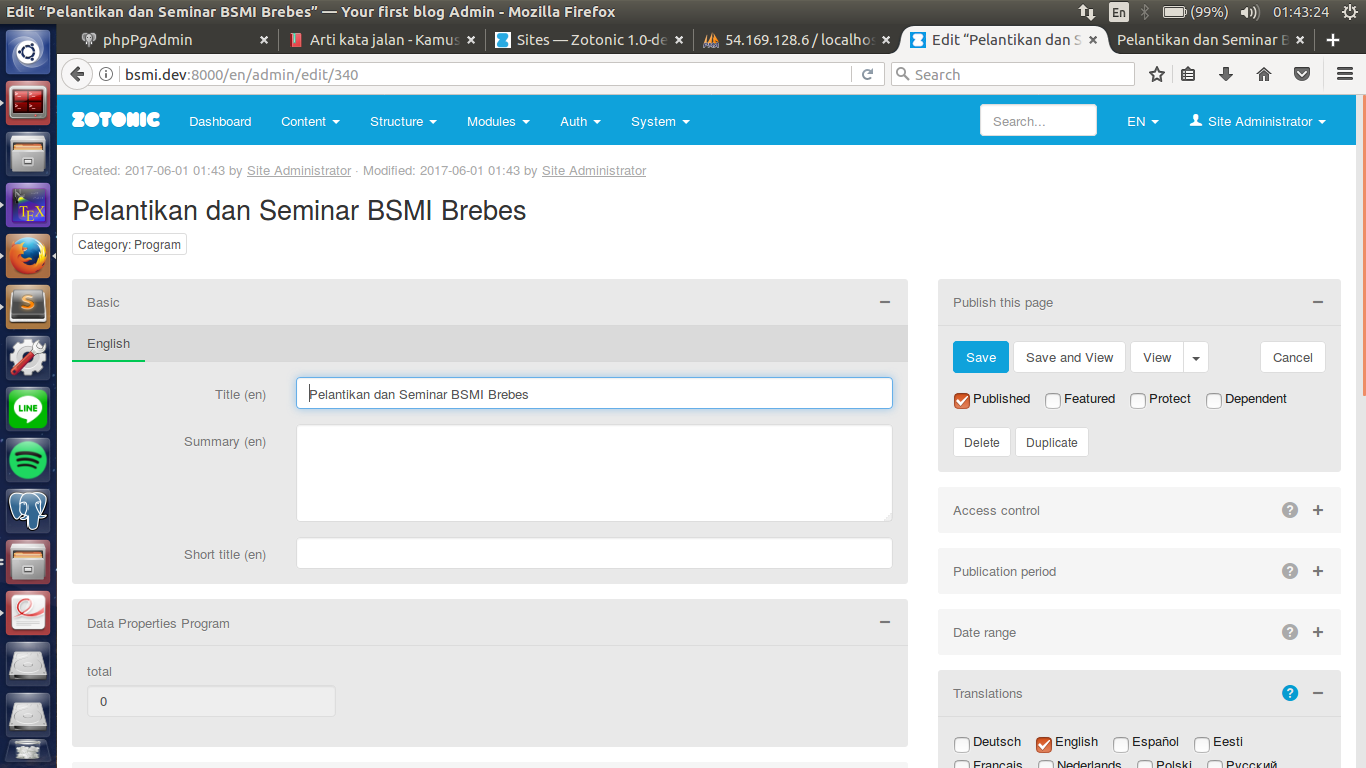
\includegraphics[width=1\textwidth]
	{pics/4-editProgram.png}
	\caption{Tampilan halaman mengubah detail \textit{page} kategori program}
	\label{fig:editprogram}
\end{figure}
\vspace{-0.3cm}

\begin{figure}
	\centering
	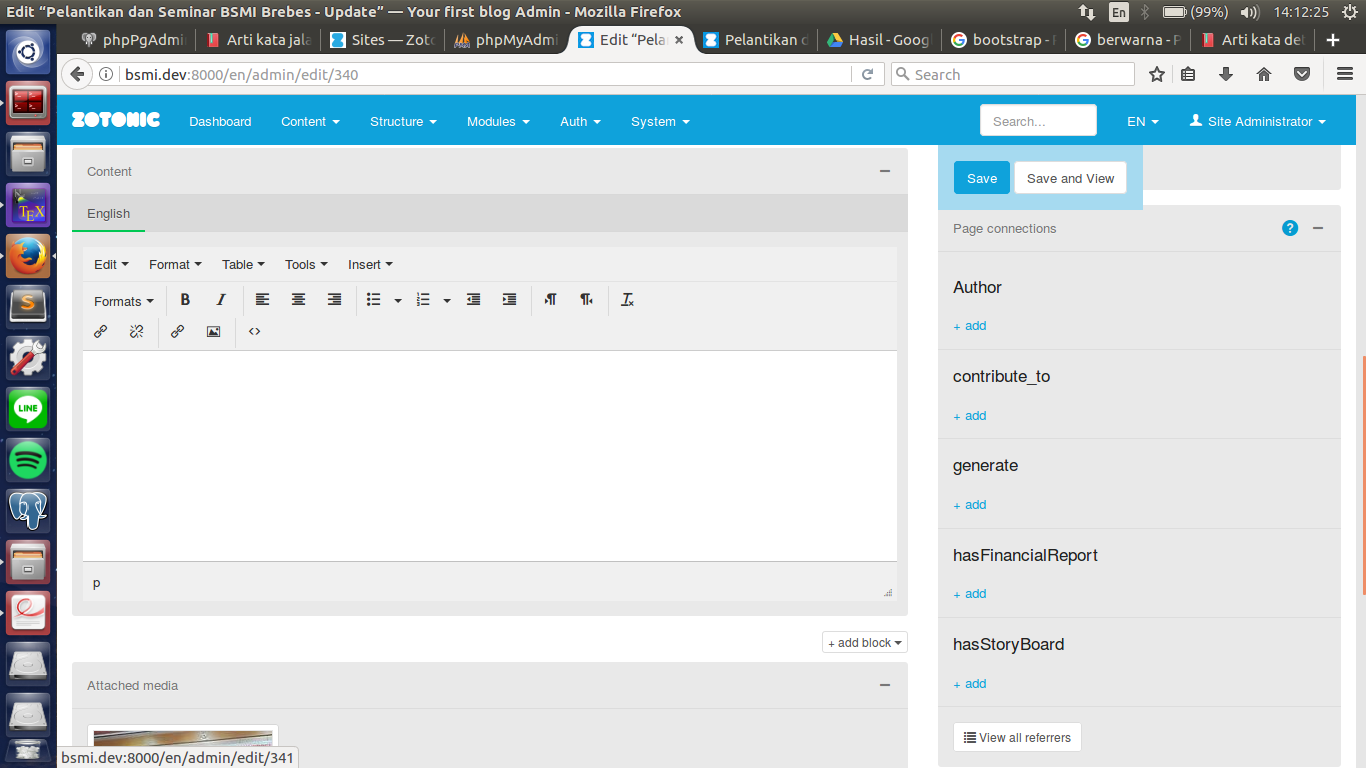
\includegraphics[width=1\textwidth]
	{pics/4-editProgram2.png}
	\caption{Tampilan halaman mengubah detail \textit{page} kategori program}
	\label{fig:editprogram2}
\end{figure}
\vspace{0.5cm}

Setelah selesai mengubah detail dari \textit{page}, pengguna dapat menyimpan perubahan yang telah dibuat dengan menekan tombol \textit{save}. Selain tersimpan pada database Zotonic, \textit{page} akan disimpan juga pada sebuah database yang didesain sesuai dengan ontologi yang ada. Penyimpanan \textit{page} ke database tersebut dengan memanfaatkan \textit{adaptor} yang telah dibuat. Pada \pic~\ref{fig:saveprogram}, dapat dilihat bahwa \textit{page} dengan judul Pelantikan dan Seminar BSMI Brebes yang memiliki id 340 yang dibuat telah tersimpan pada database tersebut. Hasil dari \textit{page} yang dibuat dapat dilihat pada \pic~\ref{fig:viewprogram}.
\begin{figure}
	\centering
	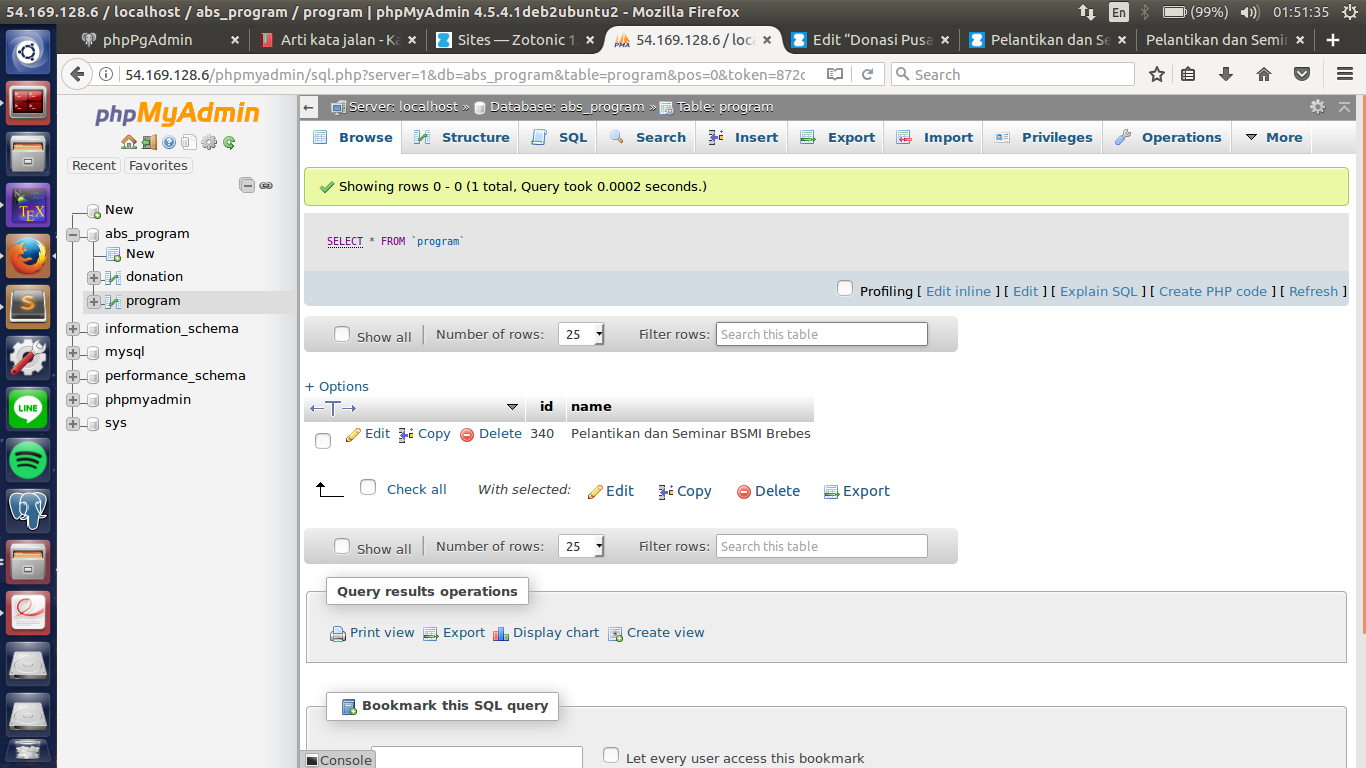
\includegraphics[width=1\textwidth]
	{pics/5-saveProgram.png}
	\caption{Penyimpanan \textit{page} program pada database eksternal}
	\label{fig:saveprogram}
\end{figure}
\vspace{-0.3cm}

\begin{figure}
	\centering
	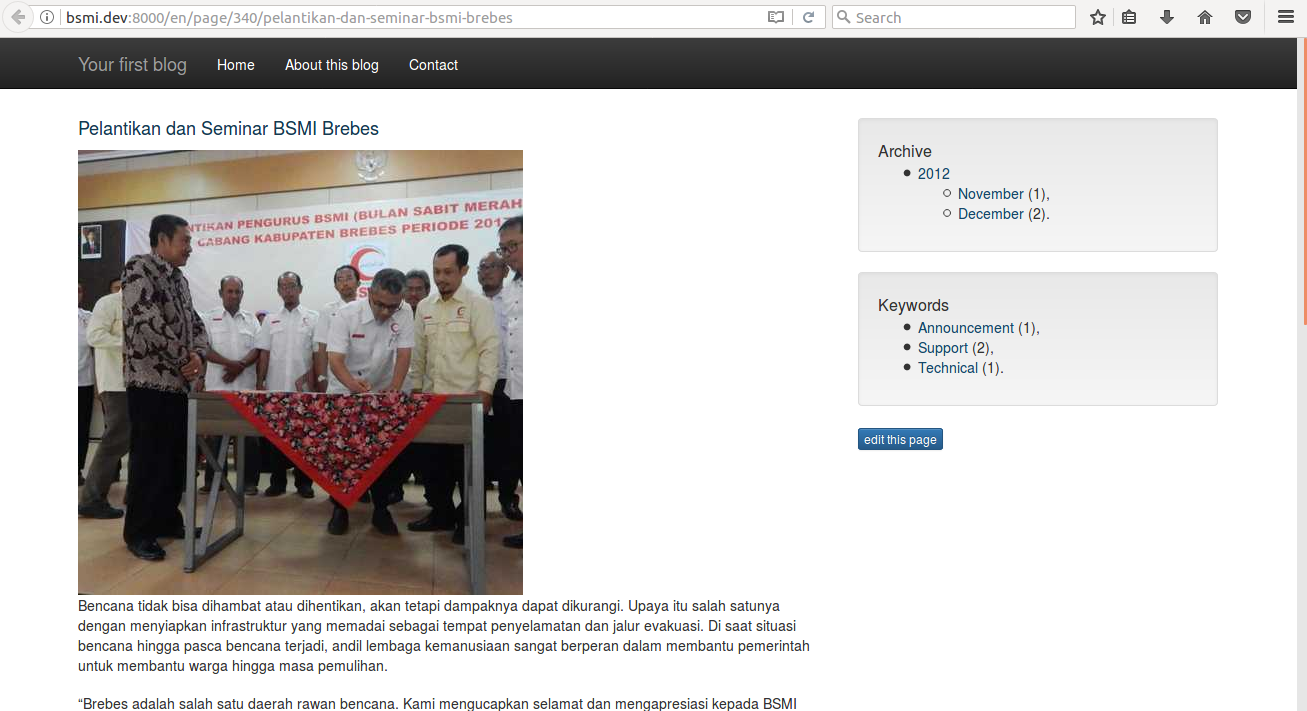
\includegraphics[width=1\textwidth]
	{pics/5-viewProgram.png}
	\caption{Tampilan \textit{page} Pelantikan dan Seminar BSMI Brebes}
	\label{fig:viewprogram}
\end{figure}
\vspace{-0.3cm}

Selanjutnya untuk mencoba \textit{business logic} yang telah diimplementasikan, perlu terlebih dahulu untuk membuat \textit{page} dengan kategori donasi. Hal ini karena setiap donasi akan terhubung dengan sebuah program sesuai dengan ontologinya. Proses pembuatan \textit{page} untuk kategori donasi hampir sama dengan proses pembuatan \textit{page} kategori lainnya yaitu dengan menekan tombol berwarna biru pada halaman \textit{dashboard} admin yang bertulisan \textit{Make a new page or media}, lalu mengisi judul dari \textit{page} yang akan dibuat dan memilih kategori \textit{donation} sebagai kategori dari \textit{page} tersebut lalu klik tombol \textit{Make page} sepert pada \pic~\ref{fig:createdonation}
\begin{figure}
	\centering
	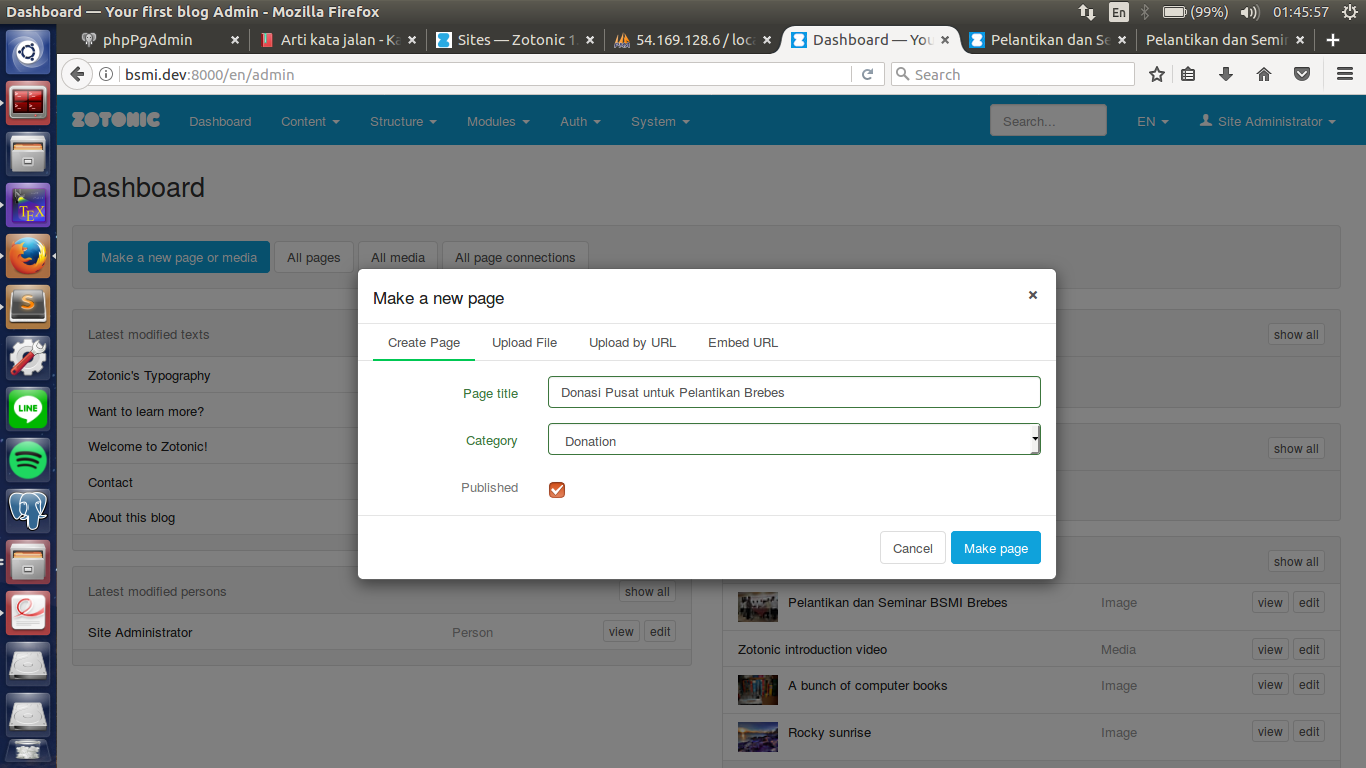
\includegraphics[width=1\textwidth]
	{pics/6-createDonation.png}
	\caption{Tampilan membuat \textit{page} pada Zotonic}
	\label{fig:createdonation}
\end{figure}
\vspace{-0.3cm}

Selanjutnya pengguna akan menuju sebuah halaman untuk mengubah detail dari \textit{page} yang sedang dibuat seperti pada \pic~\ref{fig:editdonation}. Donasi memiliki sebuah \textit{data properties} yaitu \textit{amount} dimana nilai \textit{amount} ini nantinya akan diakumulasikan menjadi nilai dari total pada program yang terhubungan dengan \textit{page} donasi ini. Untuk dapat melihat apakah \textit{business logic} sudah bekerja, maka \textit{amount} dari \textit{page} donasi harus diisi dengan angka. Seperti pada \pic~\ref{fig:editdonation2}, nilai dari \textit{amount} diisi dengan 7000000. Nilai 7000000 ini akan menjadi bagian dari nilai total program yang terkait dengan donasi ini.
\begin{figure}
	\centering
	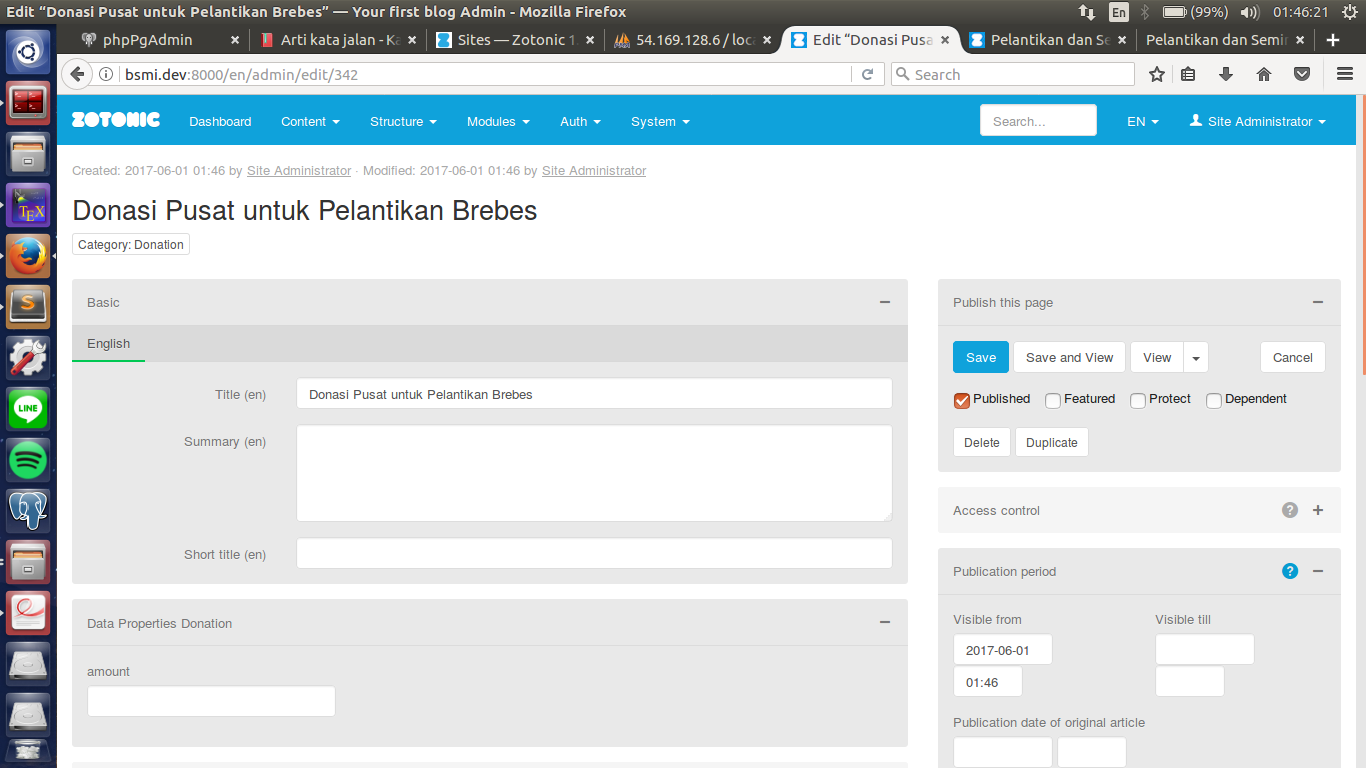
\includegraphics[width=1\textwidth]
	{pics/7-editDonation.png}
	\caption{Tampilan halaman untuk mengubah donasi pada Zotonic}
	\label{fig:editdonation}
\end{figure}
\vspace{-0.3cm}

\begin{figure}
	\centering
	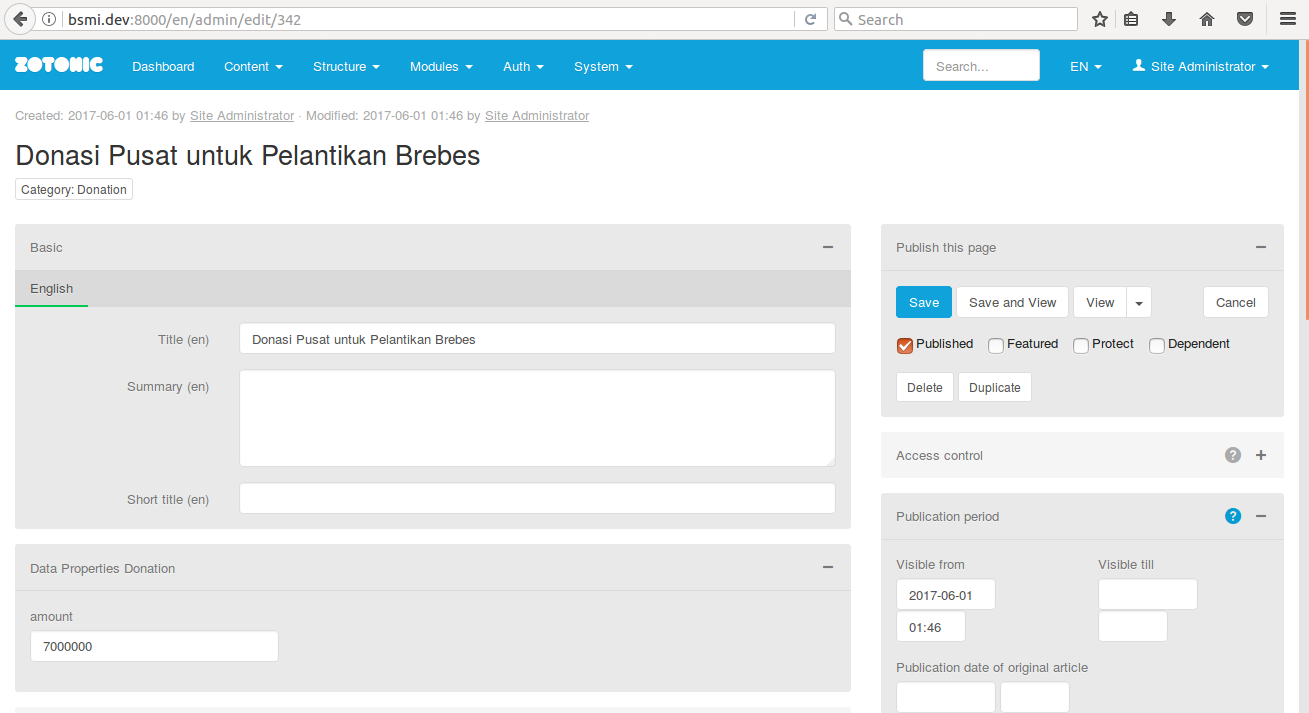
\includegraphics[width=1\textwidth]
	{pics/8-editDonation2.png}
	\caption{Tampilan halaman mengubah detail \textit{page} kategori donasi}
	\label{fig:editdonation2}
\end{figure}
\vspace{-0.3cm}

Untuk membuat koneksi antara suatu donasi dengan suatu program, maka pada bagian \textit{page connection} harus diisi koneksi \textit{forProgram} yang menggambarkan donasi ini ditujukan untuk program yang mana seperti pada \pic~\ref{fig:editdonation3}. Tekan \textit{add} pada bagian \textit{forProgram} untuk memilih program yang dituju, lalu akan muncul \textit{modals} seperti pada \pic~\ref{fig:editdonation4}.
\begin{figure}
	\centering
	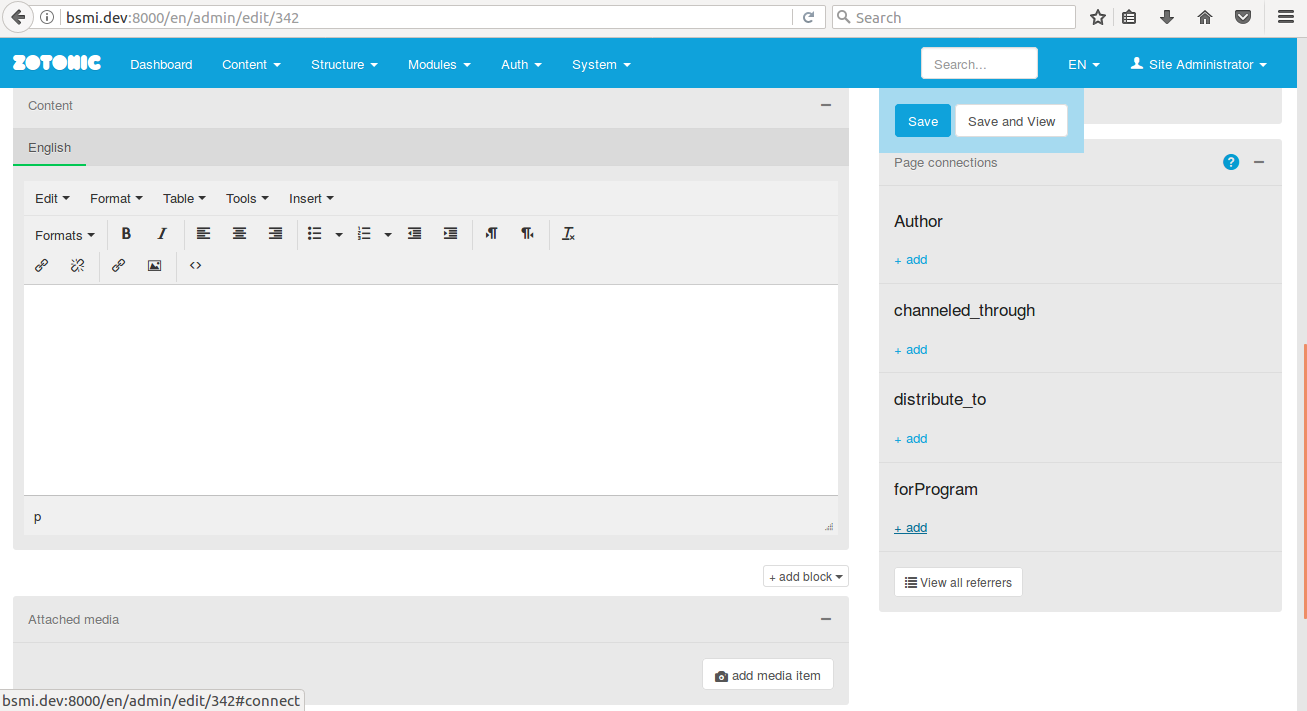
\includegraphics[width=1\textwidth]
	{pics/9-editDonation3.png}
	\caption{Tampilan halaman mengubah detail \textit{page} kategori donasi}
	\label{fig:editdonation3}
\end{figure}
\vspace{-0.3cm}

Pada \pic~\ref{fig:editdonation4}, \textit{modals} yang muncul akan menampilkan seluruh \textit{page} program yang telah ada. Pada contoh ini, karena \textit{site} baru memiliki sebuah \textit{page} dengan kategori program maka yang ditampilkan hanya satu. Dengan bantuan \textit{modals} ini, pengguna akan lebih mudah untuk menambahkan koneksi antara donasi dan program.
\begin{figure}
	\centering
	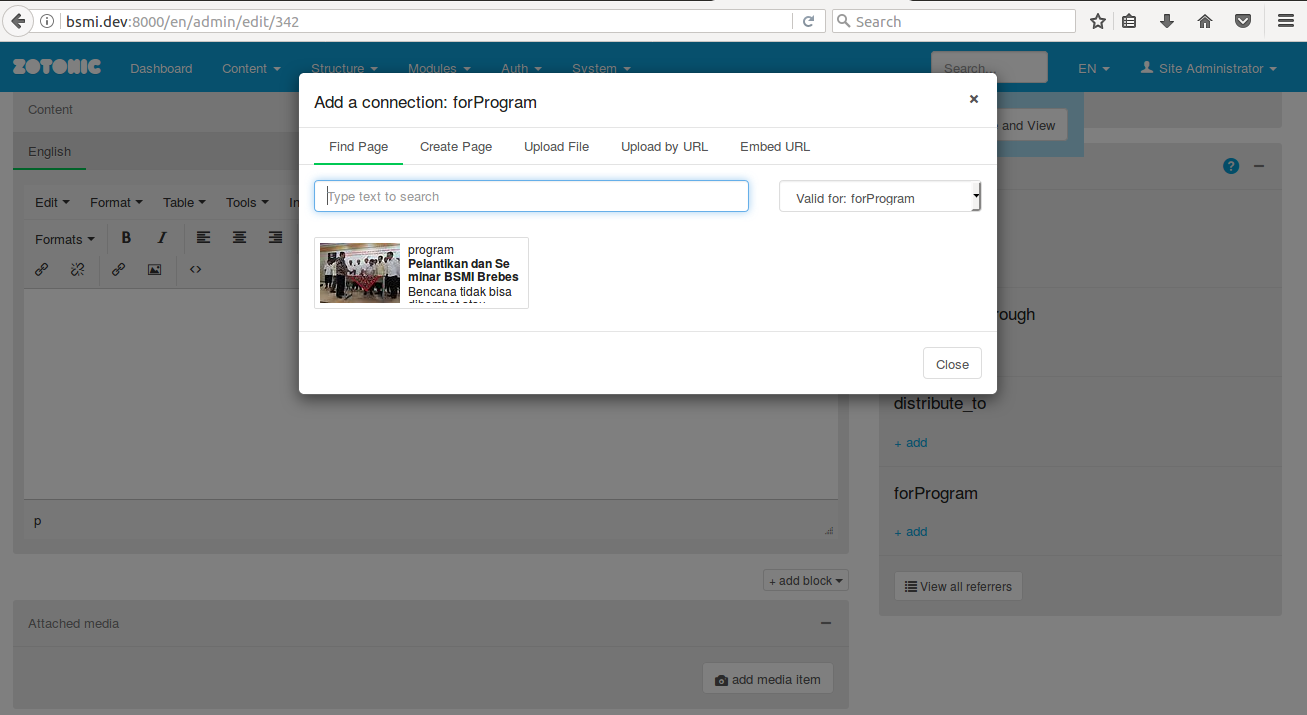
\includegraphics[width=1\textwidth]
	{pics/10-editDonation4.png}
	\caption{Tampilan halaman mengubah detail \textit{page} kategori donasi}
	\label{fig:editdonation4}
\end{figure}
\vspace{-0.3cm}

Setelah memilih program mana yang akan ditujukan untuk donasi ini, tampilannya akan menjadi seperti pada \pic~\ref{fig:editdonation5}. Lalu simpan perubahan dengan menekan tombol save.
\begin{figure}
	\centering
	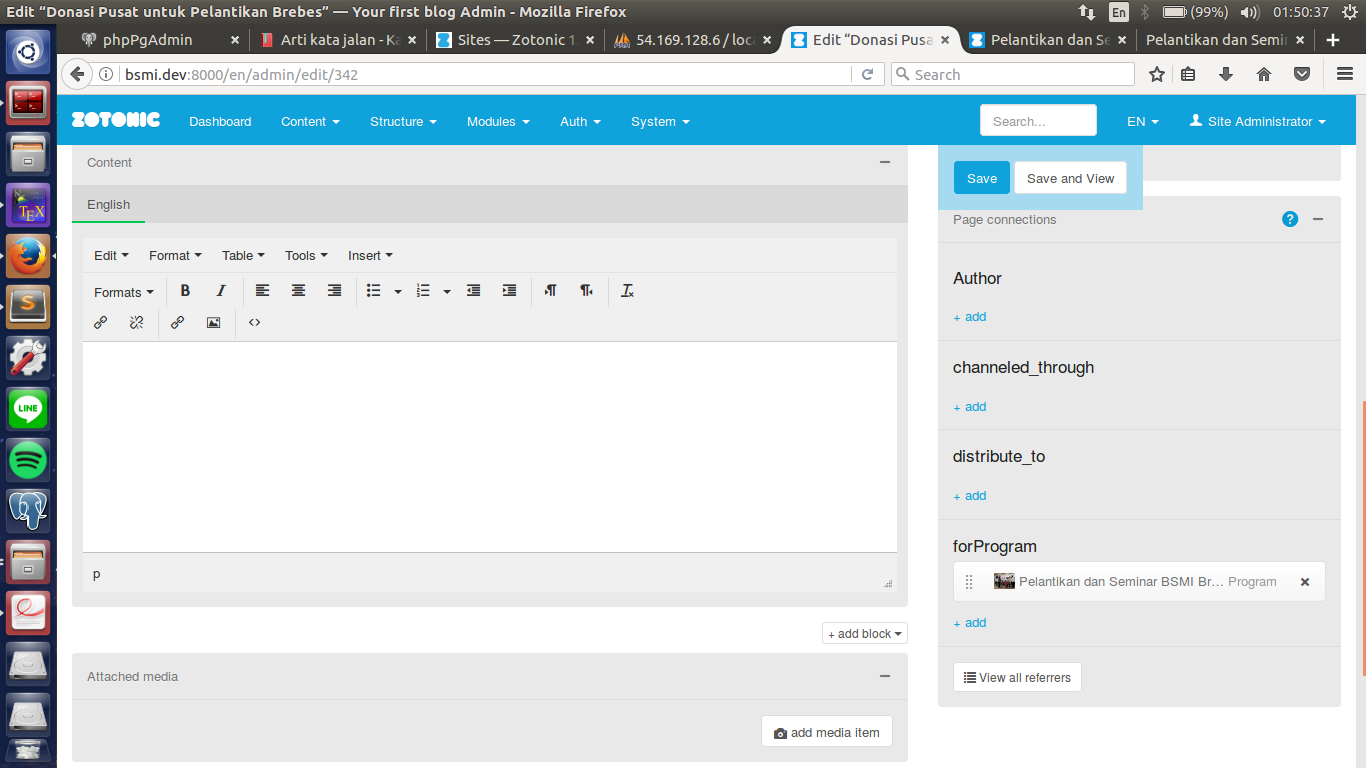
\includegraphics[width=1\textwidth]
	{pics/11-editDonation5.png}
	\caption{Tampilan halaman mengubah detail \textit{page} kategori donasi}
	\label{fig:editdonation5}
\end{figure}
\vspace{-0.3cm}

Ketika donasi tersebut disimpan, donasi tersebut akan disimpan juga pada database eksternal. Sama seperti dengan \textit{page} kategori program, \textit{page} kategori donasi juga akan disimpan ke database eksternal dengan memanfaatkan \textit{adaptor} yang sudah diimplementasikan. Pada \pic~\ref{fig:savedonation} dapat dilihat bahwa donasi dengan nama Donasi pusat untuk Pelantikan Brebes dengan amount sebesar 7000000 dan id 342 telah tersimpan. Selain itu, informasi tentang program yang terkait dengan donasi ini juga disimpan yang dilambangkan oleh p\_id. Untuk donasi ini, karena donasi dengan id 342 ditujukan untuk program Pelantikan dan Seminar BSMI Brebes yang memiliki id 340 maka p\_id dari donasi ini adalah 340.
\begin{figure}
	\centering
	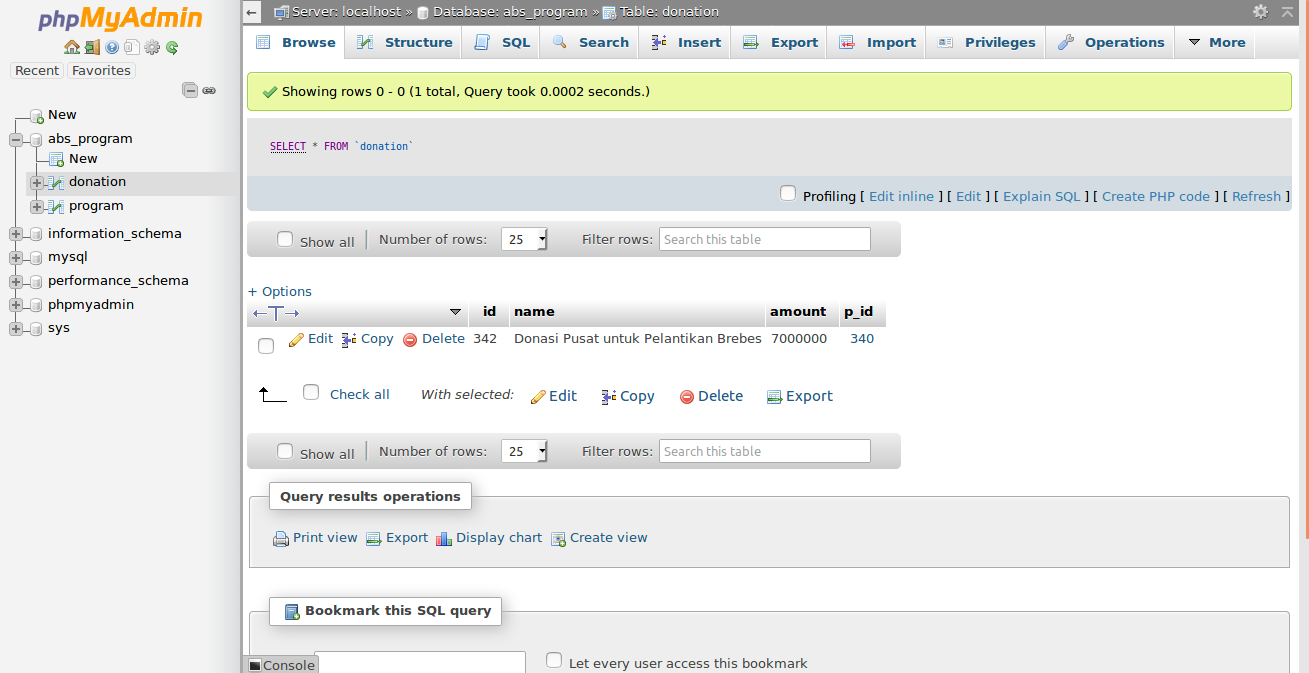
\includegraphics[width=1\textwidth]
	{pics/12-saveDonation.png}
	\caption{Penyimpanan donasi pada database eksternal}
	\label{fig:savedonation}
\end{figure}
\vspace{-0.3cm}

Setelah pembuatan donasi yang ditujukan untuk program Pelantikan dan Seminar BSMI Brebes, maka terjadi perubahan pada halaman program Pelantikan dan Seminar BSMI Brebes yaitu tampilnya nilai dari total donasi untuk program tersebut yang dapat dilihat pada \pic~\ref{fig:viewprogram2}. Perhitungan jumlah donasi tersebut telah memanfaatkan \textit{adaptor} yang telah diimplementasikan.
\begin{figure}
	\centering
	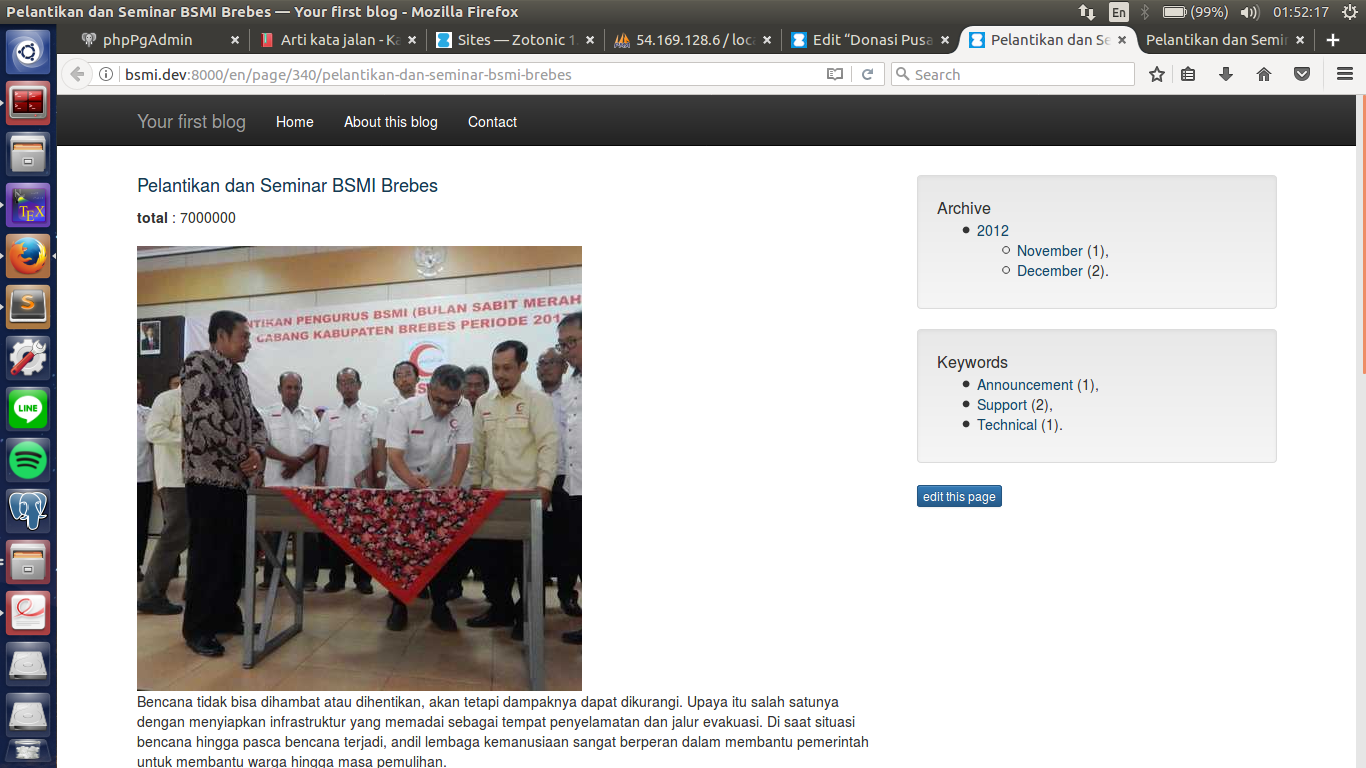
\includegraphics[width=1\textwidth]
	{pics/12-viewprogram.png}
	\caption{Tampilan \textit{page} Pelantikan dan Seminar BSMI Brebes setelah pembuatan donasi}
	\label{fig:viewprogram2}
\end{figure}
\vspace{-0.3cm}

Agar lebih dapat terlihat apakah \textit{business logic} untuk total donasi telah benar, maka ditambahkan lagi donasi baru untuk program Pelantikan dan Seminar BSMI Brebes. Sama seperti pembuatan donasi sebelumnya, langkah pembuatan donasi baru dengan menekan tombol \textit{Make a new page or media} pada halaman \textit{dashboard} admin. Lalu akan muncul \textit{modals}. Pada \textit{modals} tersebut perlu diisi nama dari donasi yang akan dibuat dan kategorinya dipilih \textit{donation} seperti \pic~\ref{fig:createdonation2}. Setelah selesai mengisi informasi tersebut, dapat menekan tombol \textit{Make page} pada \textit{modals} tersebut.
\begin{figure}
	\centering
	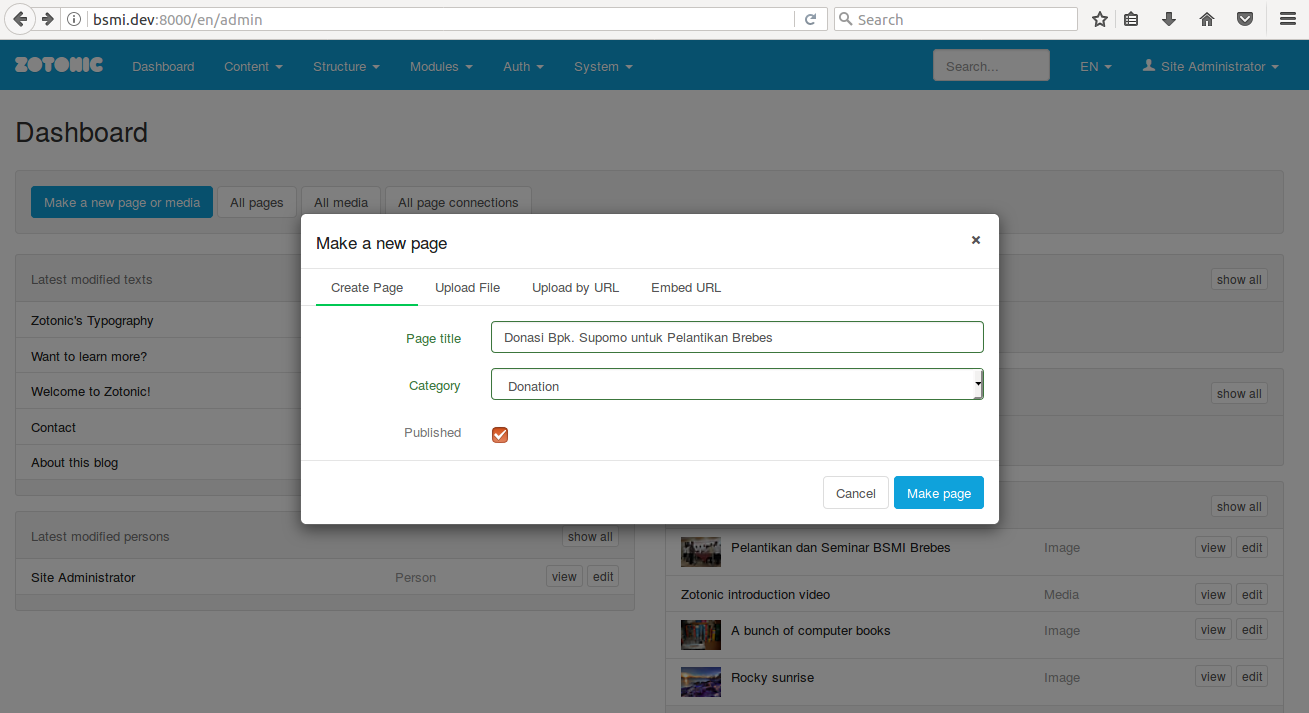
\includegraphics[width=1\textwidth]
	{pics/13-createDonation2.png}
	\caption{Tampilan membuat \textit{page} pada Zotonic}
	\label{fig:createdonation2}
\end{figure}
\vspace{-0.3cm}

Setelah menekan tombol \textit{Make page} pada \textit{modals} tersebut, pengguna akan diarahkan menuju halaman untuk mengubah detail dari \textit{page} yang sedang dibuat seperti pada \pic~\ref{fig:edit2donation}. Sama seperti pada proses pembuatan \textit{page} donasi sebelumnnya, pengguna harus memasukkan nilai \textit{amount} dari donasi pada \textit{data properties} seperti \pic~\ref{fig:edit2donation2}.
\begin{figure}
	\centering
	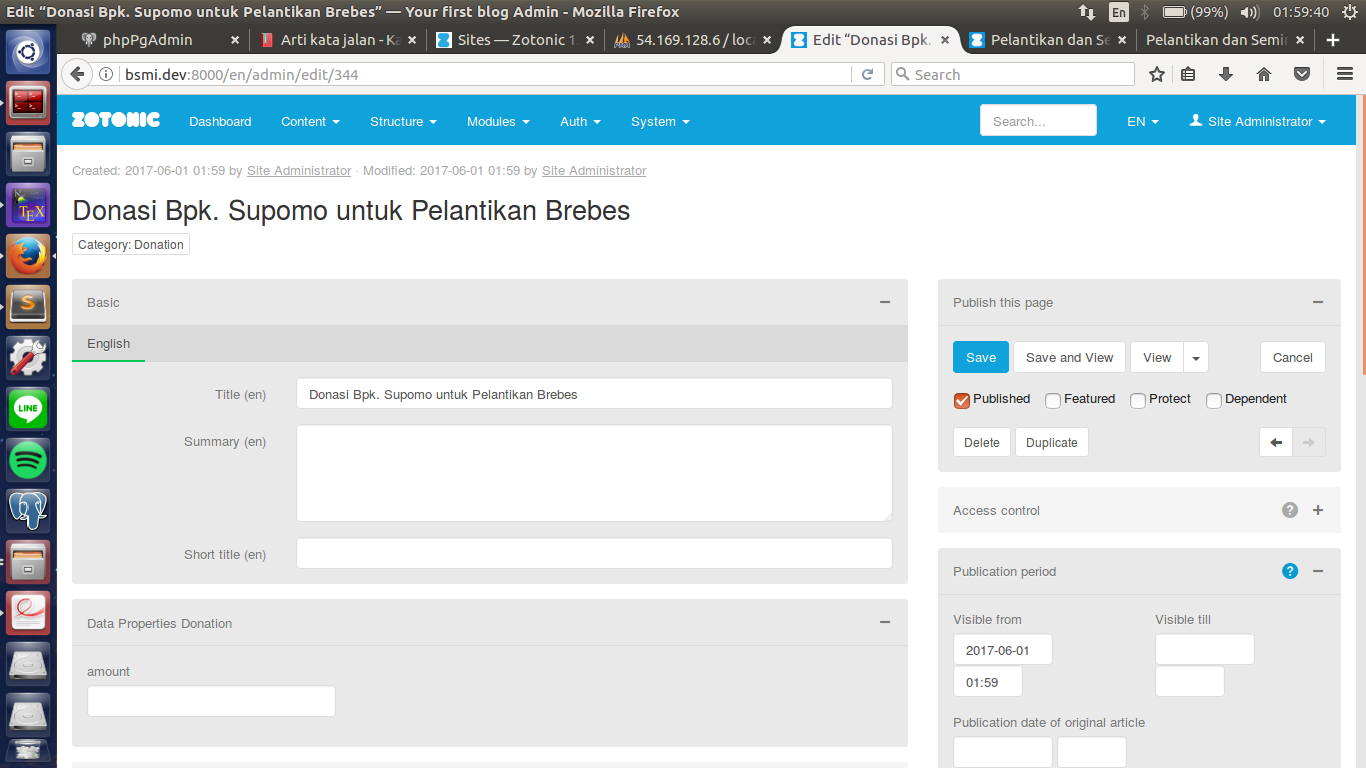
\includegraphics[width=1\textwidth]
	{pics/14-edit2Donation.png}
	\caption{Tampilan halaman mengubah detail \textit{page} pada kategori Donasi}
	\label{fig:edit2donation}
\end{figure}
\vspace{-0.3cm}

Untuk donasi dengan judul Donasi Bpk. Supomo untuk Pelantikan Brebes, nilai \textit{amount} diberi 750000 seperti \pic~\ref{fig:edit2donation2}. Setelah mengisi nilai \textit{amount}, selanjutnya pengguna harus menghubungkan donasi dengan suatu program. Untuk melakukan hal tersebut, tekan tombol \textit{add} \textit{forProgram} pada \textit{page connection}.
\begin{figure}
	\centering
	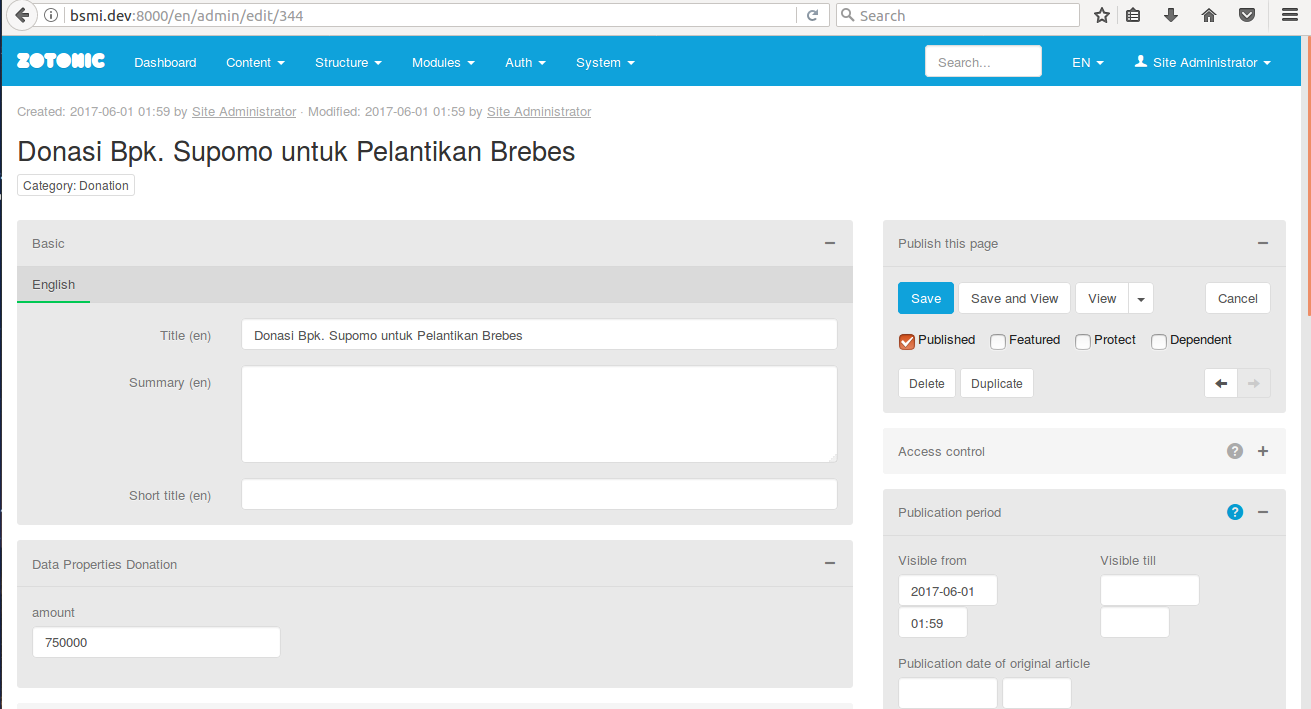
\includegraphics[width=1\textwidth]
	{pics/15-edit2Donation2.png}
	\caption{Tampilan halaman mengubah detail \textit{page} pada kategori Donasi}
	\label{fig:edit2donation2}
\end{figure}
\vspace{-0.3cm}

Lalu akan muncul sebuah \textit{modals} yang menampilkan seluruh program yang ada seperti pada \pic~\ref{fig:edit2donation3}. Pilih program mana yang akan dituju, lalu tekan tombol \textit{close} sehingga akan muncul tampilan seperti \pic~\ref{fig:edit2donation4}. Setelah proses perubahan selesai dilakukan, tekan tombol \textit{save} untuk menyimpan perubahan yang telah dibuat.
\begin{figure}
	\centering
	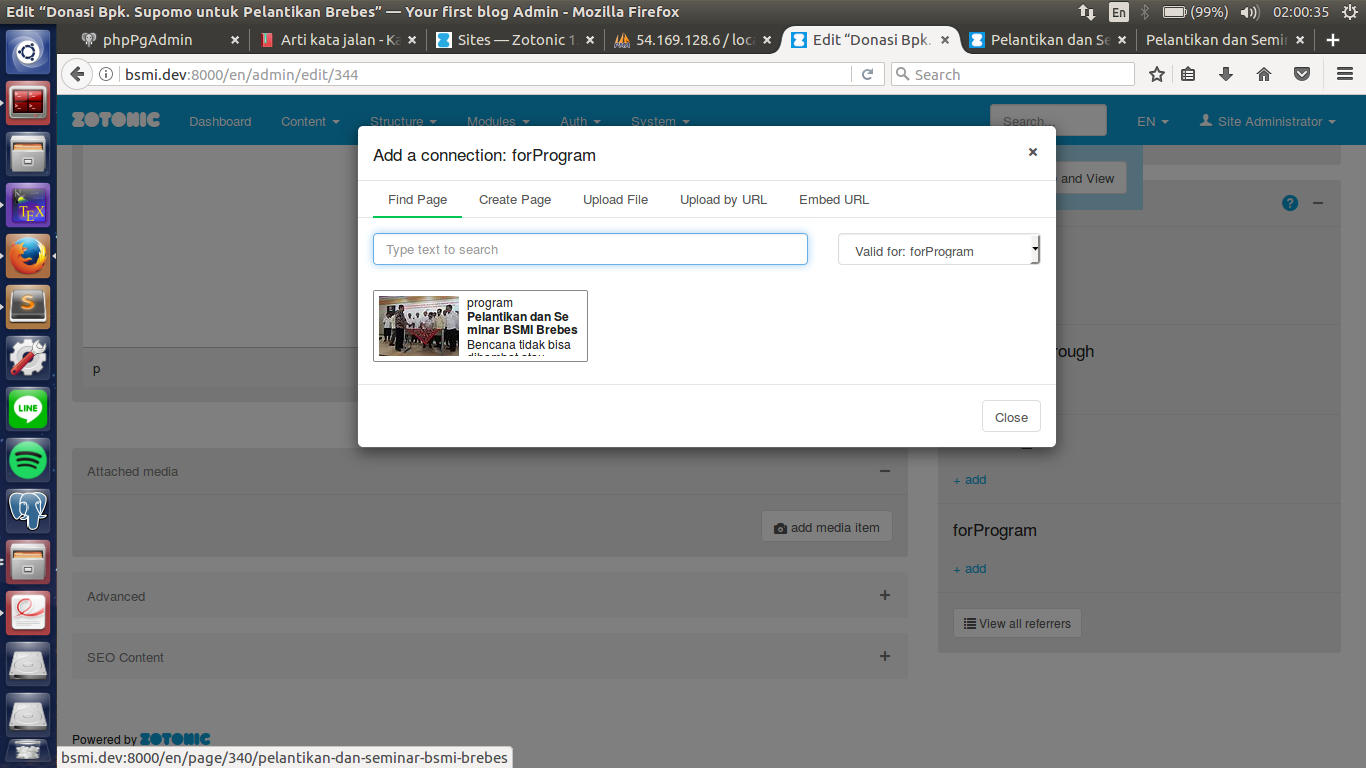
\includegraphics[width=1\textwidth]
	{pics/16-edit2Donation3.png}
	\caption{Tampilan halaman mengubah detail \textit{page} pada kategori Donasi}
	\label{fig:edit2donation3}
\end{figure}
\vspace{-0.3cm}

\begin{figure}
	\centering
	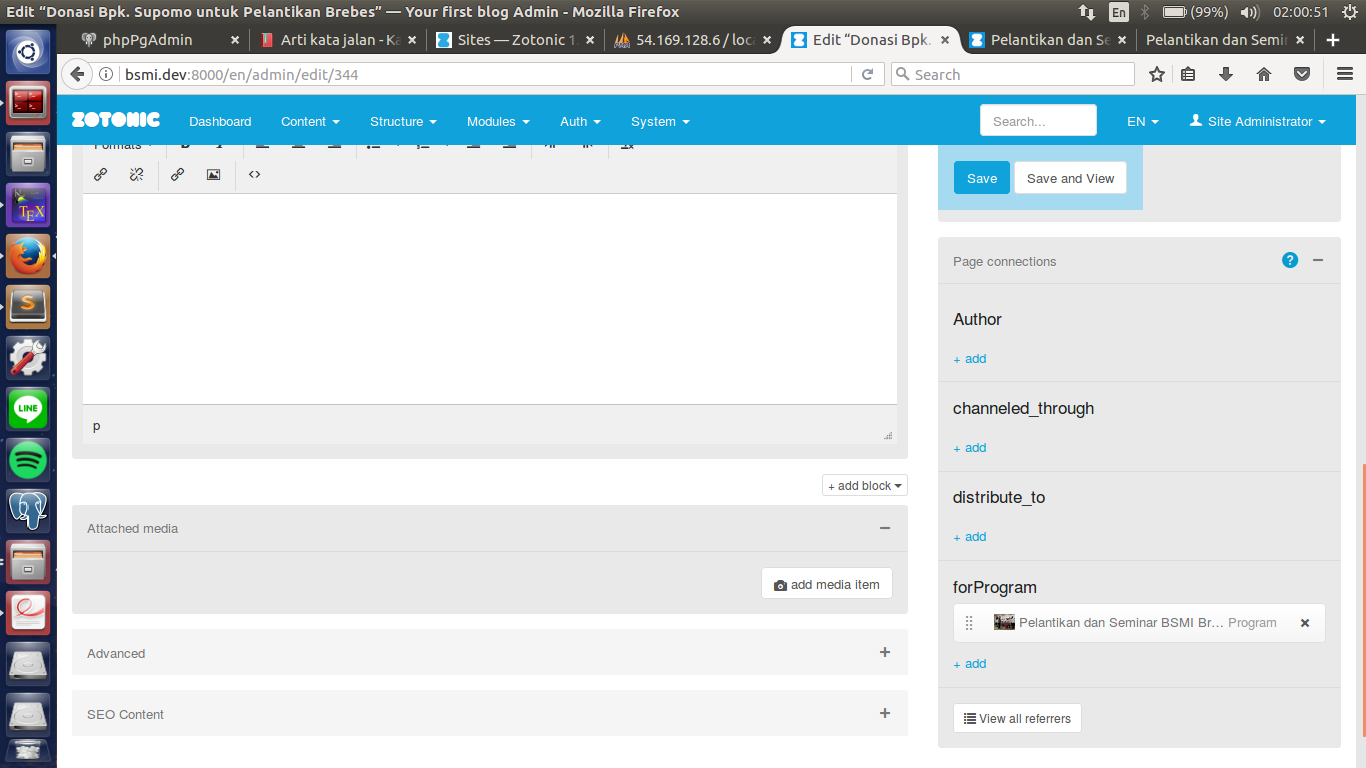
\includegraphics[width=1\textwidth]
	{pics/17-edit2Donation4.png}
	\caption{Tampilan halaman mengubah detail \textit{page} pada kategori Donasi}
	\label{fig:edit2donation4}
\end{figure}
\vspace{-0.3cm}

Sama seperti donasi sebelumnya, ketika sebuah donasi disimpan maka akan tersimpan juga pada database eksternal dengan memanfaatkan \textit{adaptor} yang telah diimplementasi. Hal ini dapat dilihat pada \pic~\ref{fig:edit2donation4} dimana donasi dengan judul Donasi Bpk. Supomo untuk Pelantikan Brebes yang memiliki id 344 dan \textit{amount} 750000 telah tersimpan pada database eksternal. Karena donasi ini ditujukan untuk program Pelantikan dan Seminar BSMI Brebes yang memiliki id 340, maka p\_id dari donasi ini adalah 340.
\begin{figure}
	\centering
	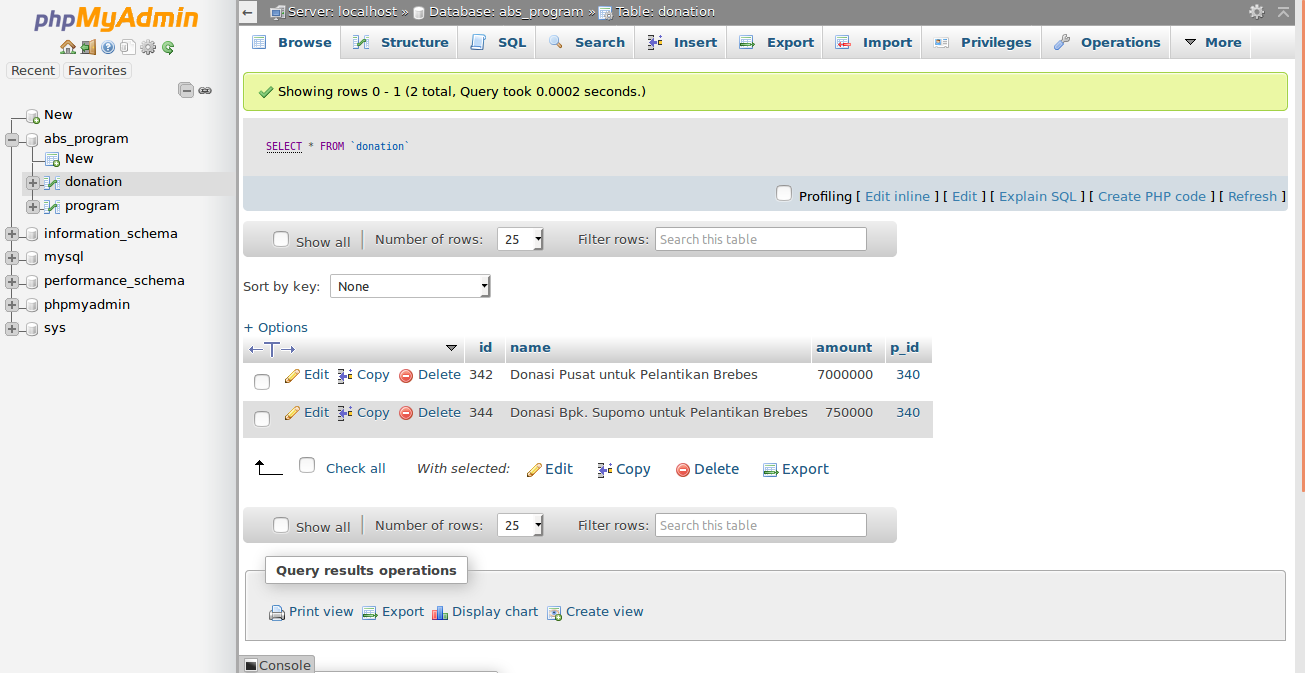
\includegraphics[width=1\textwidth]
	{pics/18-dbdonation.png}
	\caption{Penyimpanan donasi pada database eksternal}
	\label{fig:dbdonation}
\end{figure}
\vspace{-0.3cm}

Setelah donasi kedua berhasil disimpan, maka total donasi untuk program "Pelantikan dan Seminar BSMI Brebes" akan berubah menjadi 7750000 dimana donasi "Donasi Pusat untuk Pelantikan Brebes" sebesar 7000000 dan donasi "Donasi Bpk. Sutomo untuk Pelantikan Brebes" sebesar 750000. Hal ini dapat dilihat pada \textit{page} Pelantikan dan Seminar BSMI Brebes seperti pada \pic~\ref{fig:viewprogram3} dimana totalnya sudah berubah menjadi 7750000.
\begin{figure}
	\centering
	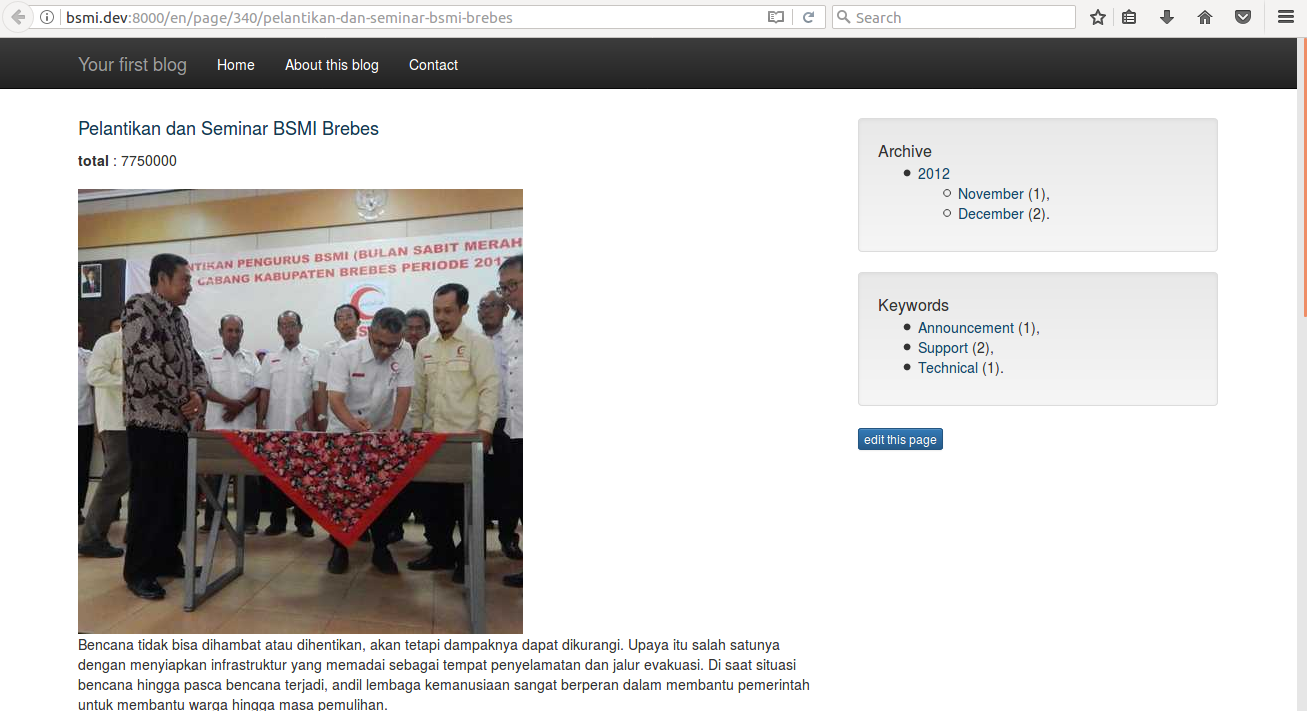
\includegraphics[width=1\textwidth]
	{pics/19-viewProgram.png}
	\caption{Tampilan \textit{page} Pelantikan dan Seminar BSMI Brebes setelah penambahan donasi}
	\label{fig:viewprogram3}
\end{figure}
\vspace{-0.3cm}

Selain pada \textit{page} Pelantikan dan Seminar BSMI Brebes, perubahan juga terjadi pada halaman untuk mengubah detail \textit{page} untuk program tersebut. Seperti pada \pic~\ref{fig:editprogramafter}, total yang terletak pada \textit{data properties} telah berubah menjadi 7750000 secara otomatis. Hal ini karena total menggunakan \textit{business logic} yang telah diimplementasikan.
\begin{figure}
	\centering
	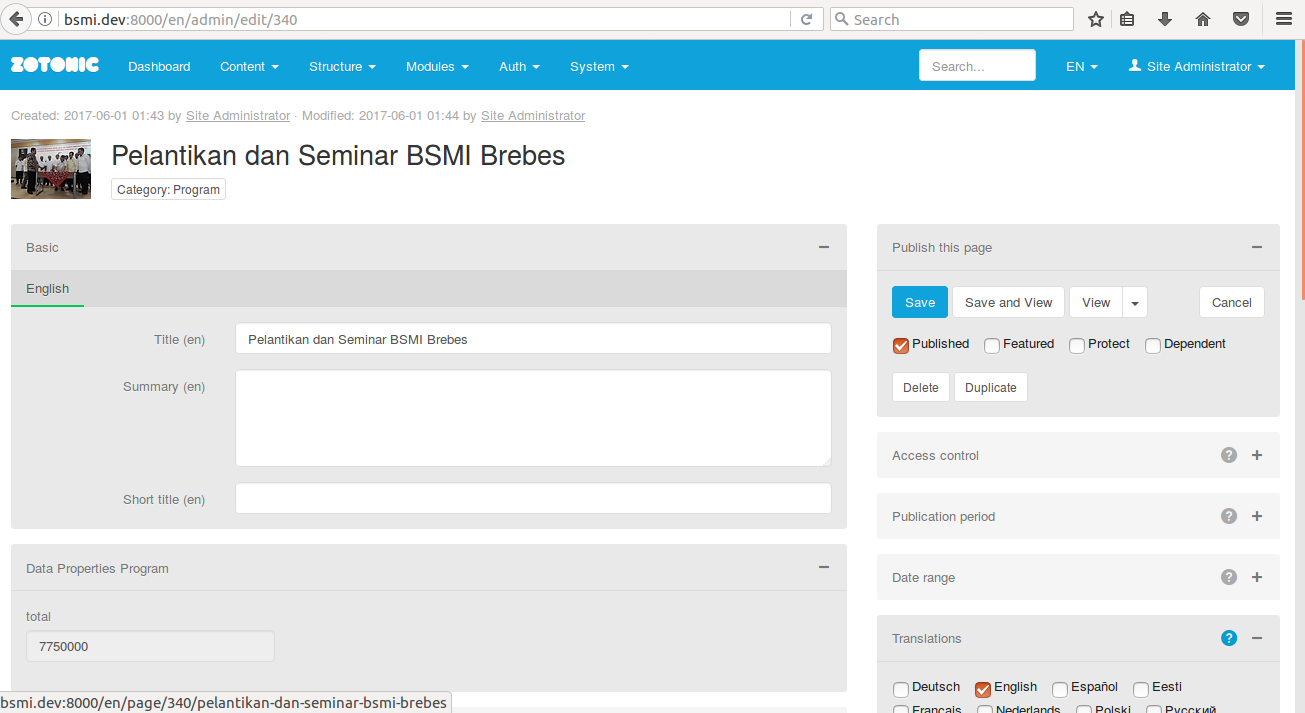
\includegraphics[width=1\textwidth]
	{pics/20-editProgramAfter.png}
	\caption{Tampilan halaman mengubah detail \textit{page} kategori program setelah ada donasi}
	\label{fig:editprogramafter}
\end{figure}
\vspace{-0.3cm}

Kasus pengujian berikutnya adalah menghapus donasi yang sudah ada untuk mengecek apakah \textit{business logic} dapat menyesuaikan dengan perubahan yang terjadi atau tidak. Setelah membuka halaman untuk mengubah detail \textit{page} dari donasi yang ingin dihapus seperti pada \pic~\ref{fig:deletedonation}, tekan tombol \textit{delete} untuk menghapus \textit{page}. Setelah menekan tombol \textit{delete}, akan muncul konfirmasi apakah ingin melanjutkan penghapusan \textit{page} atau membatalkannya. Hal ini dapat dilihat pada \pic~\ref{fig:deletedonation2}. Tekan tombol \textit{delete} untuk menghapus \textit{page} tersebut.
\begin{figure}
	\centering
	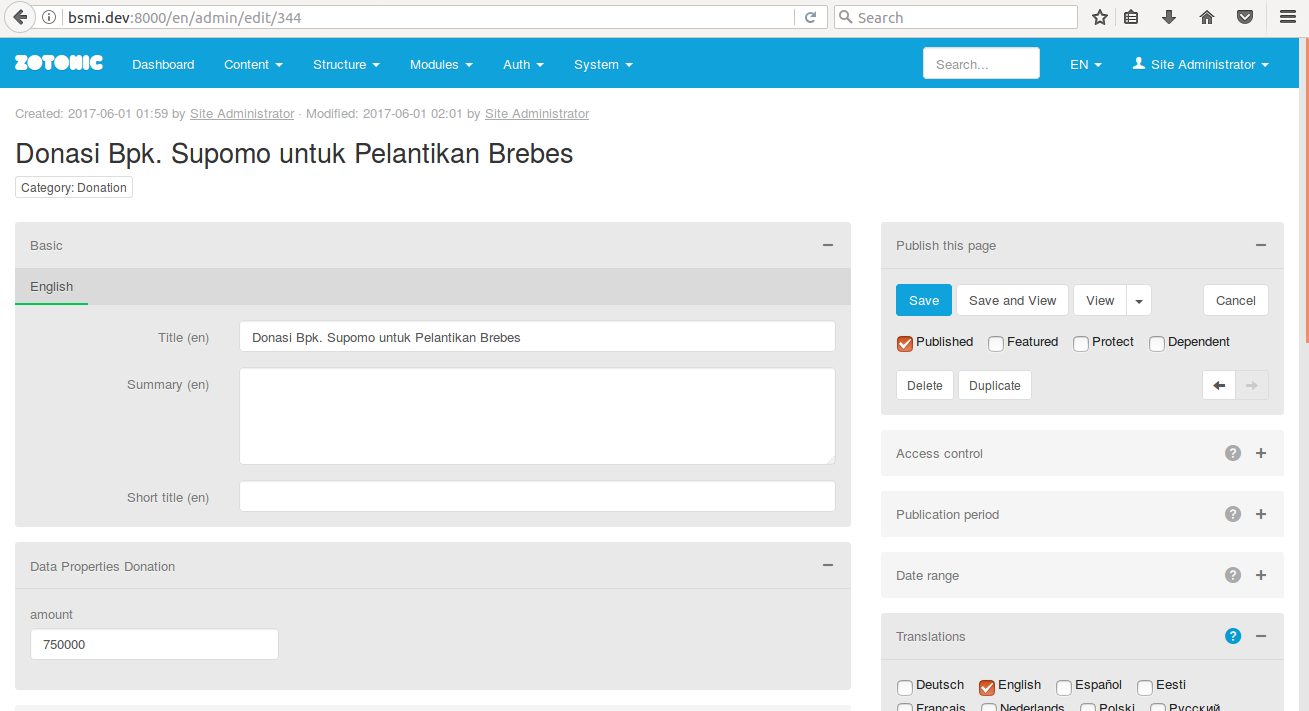
\includegraphics[width=1\textwidth]
	{pics/22-deleteDonation.png}
	\caption{Tampilan halaman mengubah detail \textit{page} pada kategori Donasi}
	\label{fig:deletedonation}
\end{figure}
\vspace{-0.3cm}

\begin{figure}
	\centering
	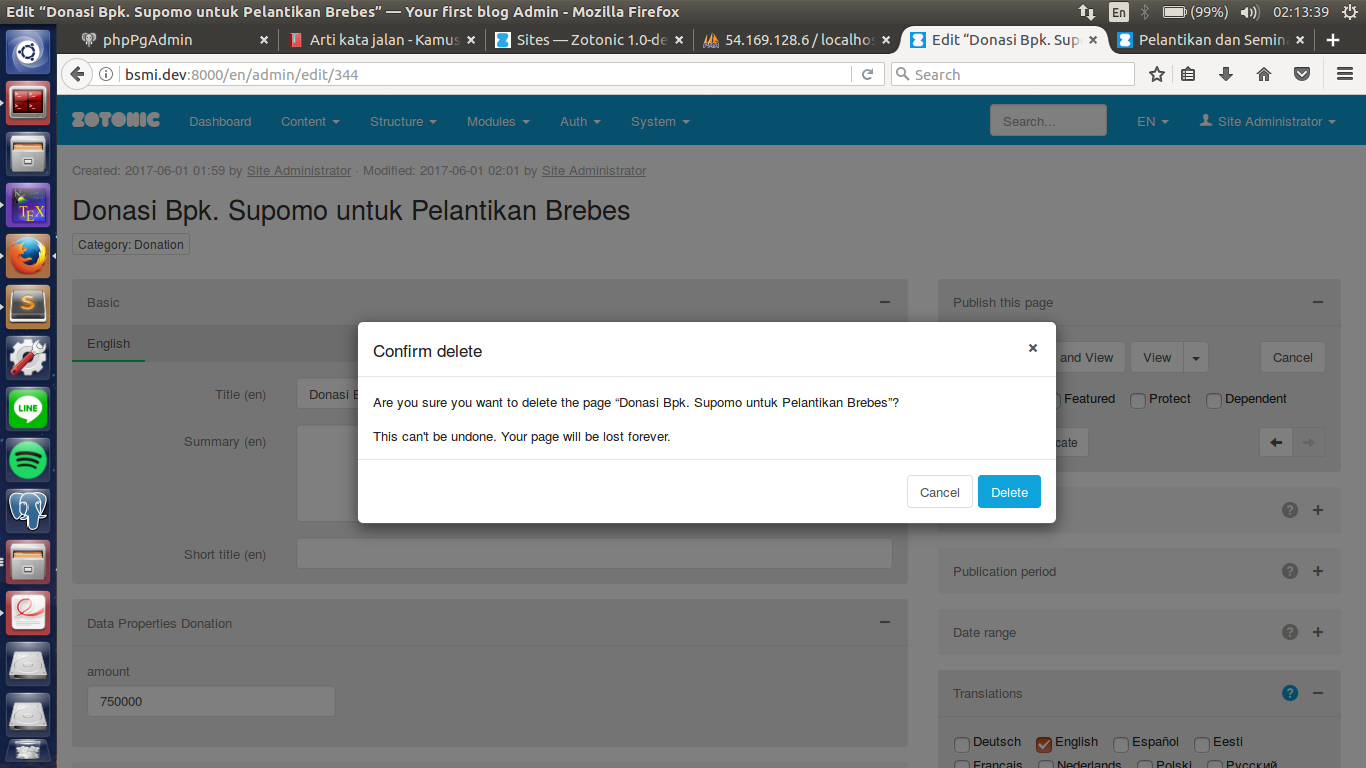
\includegraphics[width=1\textwidth]
	{pics/23-deleteDonation.png}
	\caption{Tampilan konfirmasi penghapusan \textit{page}}
	\label{fig:deletedonation2}
\end{figure}
\vspace{-0.3cm}

Ketika donasi telah berhasil dihapus, \textit{adaptor} akan melakukan penghapusan donasi yang terletak pada database eksternal sesuai dengan id dari donasi yang dihapus. Hal ini dapat dilihat pada \pic~\ref{fig:dbdelete} dimana donasi dengan id 344 sudah tidak ada lagi.
\begin{figure}
	\centering
	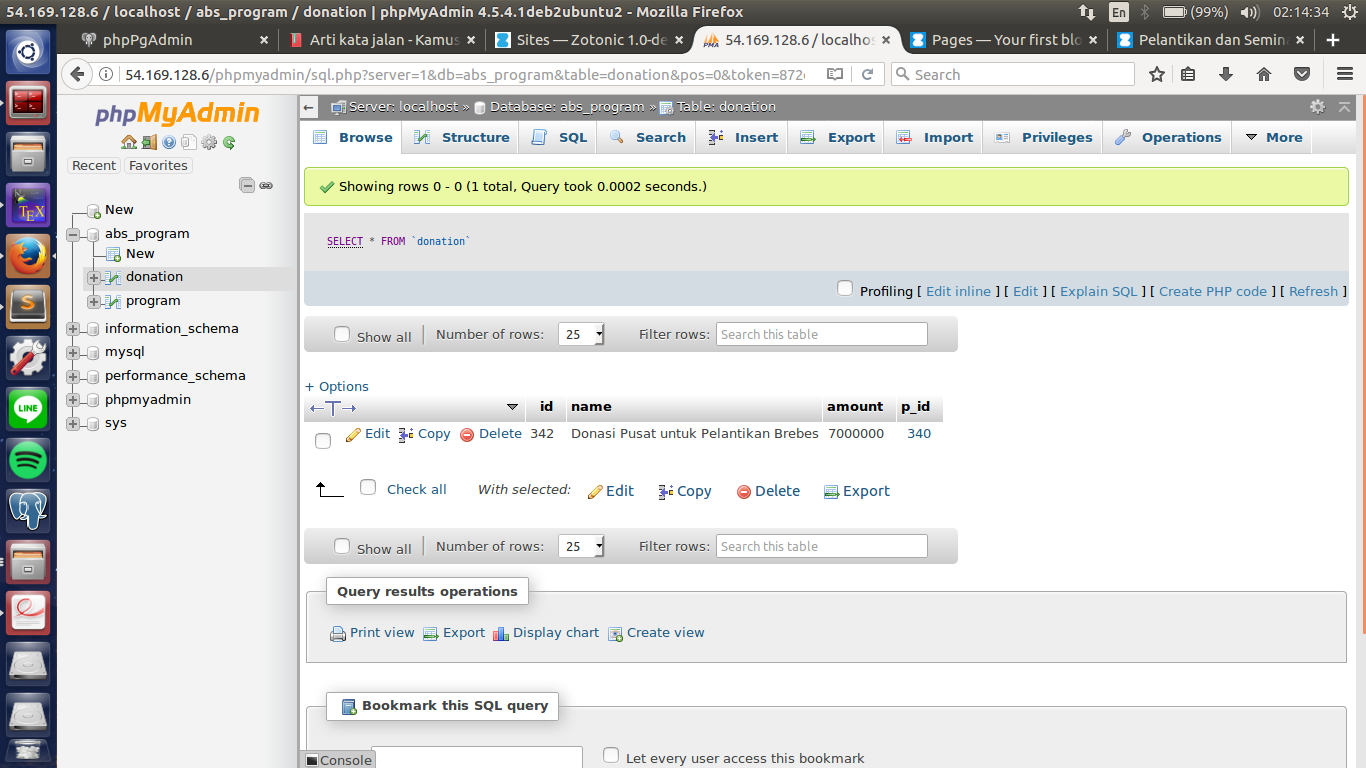
\includegraphics[width=1\textwidth]
	{pics/25-dbdelete.png}
	\caption{Penghapusan tupel pada database eksternal setelah penghapusan donasi}
	\label{fig:dbdelete}
\end{figure}
\vspace{-0.3cm}

Hal ini juga akan mengubah jumlah total donasi yang diberikan kepada program "Pelantikan dan Seminar BSMI Brebes" karena penghapusan donasi "Donasi Bpk. Supomo untuk Pelantikan Brebes". Donasi yang terhubungan dengan progam tersebut hanya tinggal donasi "Donasi Pusat untuk Pelantikan Brebes" yang memiliki \textit{amount} 7000000 sehingga total donasi yang diterima oleh program tersebut akan menjadi 7000000 juga. Untuk melihat apakah perubahannya telah terjadi atau tidak, dapat mengakses halaman dari Pelantikan dan Seminar BSMI Brebes. Pada \pic~\ref{fig:viewprogram4}, yang merupakan tampilan halaman Pelantikan dan Seminar BSMI Brebes setelah penghapusan donasi "Donasi Bpk. Supomo untuk Pelantikan Brebes", dapat dilihat bahwa total donasi sudah berubah menjadi 7000000
\begin{figure}
	\centering
	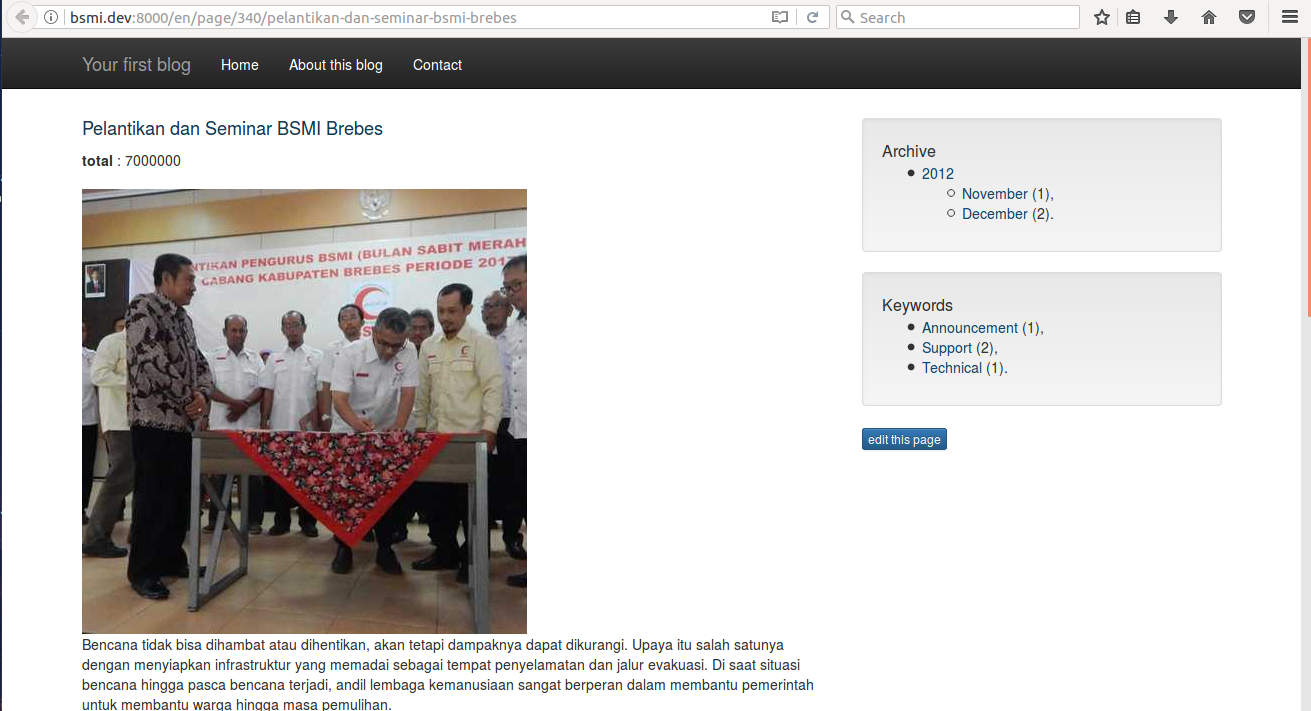
\includegraphics[width=1\textwidth]
	{pics/24-viewProgram.png}
	\caption{Tampilan \textit{page} Pelantikan dan Seminar BSMI Brebes setelah penghapusan donasi}
	\label{fig:viewprogram4}
\end{figure}
\vspace{-0.3cm}

Pengujian berikutnya adalah untuk mencoba jika suatu donasi yang sudah ada dilakukan perubahan terhadap nilai dari \textit{amount} apakah \textit{business logic} akan berubah juga. Untuk melakukan hal tersebut, buka halaman untuk mengubah detail dari donasi yang akan diubah. Pada kasus ini, penulis akan mengubah donasi "Donasi Pusat untuk Pelantikan Brebes". Seperti pada \pic~\ref{fig:updatedonation}, penulis mengubah nilai \textit{amount} donasi tersebut dari 7000000 menjadi 5000000. Selanjutnya tekan tombol \textit{save} untuk menyimpan perubahan yang terjadi.
\begin{figure}
	\centering
	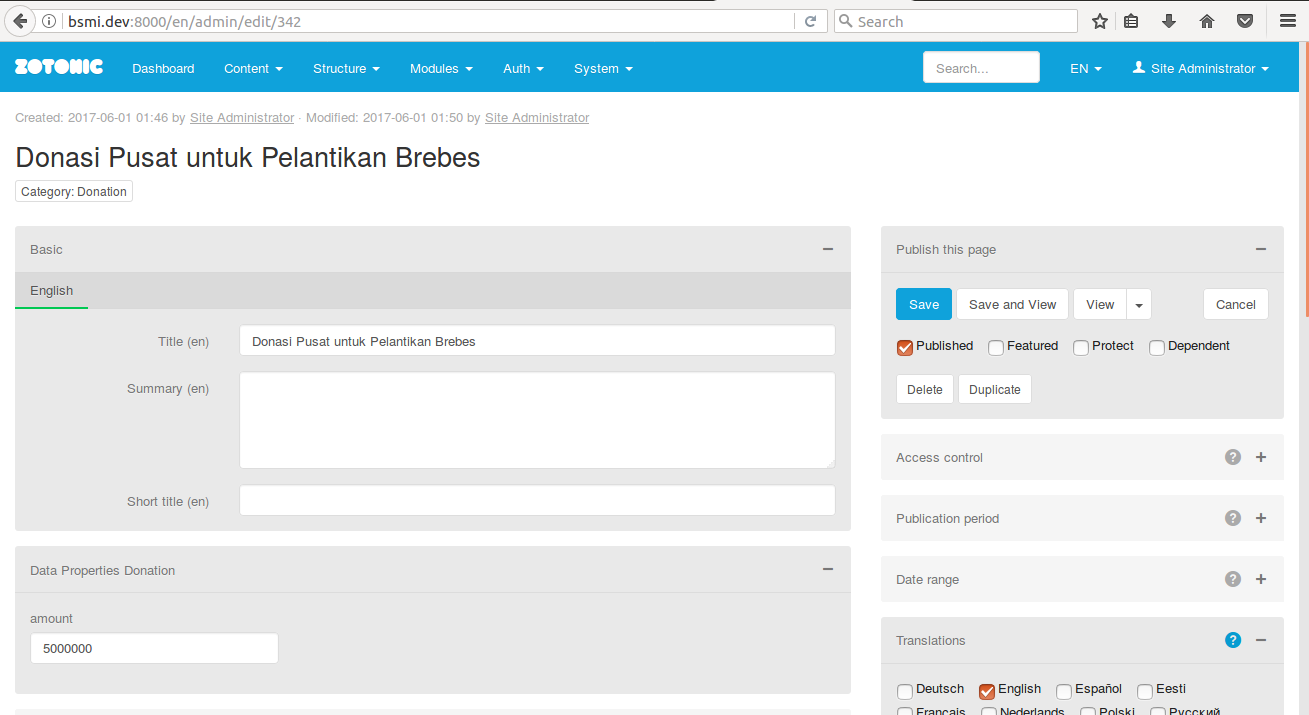
\includegraphics[width=1\textwidth]
	{pics/28-updateDonation.png}
	\caption{Tampilan halaman mengubah detail \textit{page} pada kategori Donasi}
	\label{fig:updatedonation}
\end{figure}
\vspace{-0.3cm}

Ketika perubahan berhasil disimpan, maka perubahan tersebut akan tersimpan juga pada database eksternal. Seperti pada \pic~\ref{fig:dbupdatedonation}, terlihat bahwa donasi dengan id 342 dimana nilai dari \textit{amount} telah berubah menjadi 5000000.
\begin{figure}
	\centering
	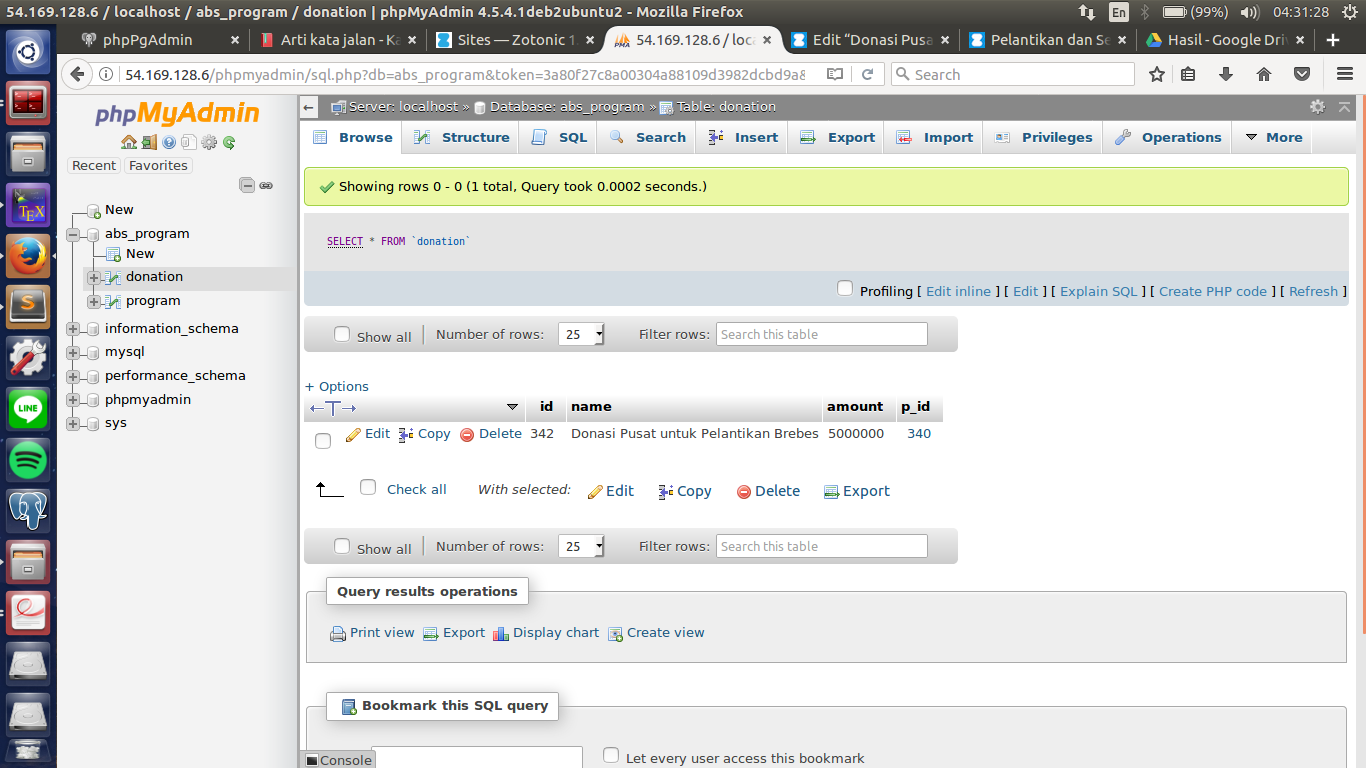
\includegraphics[width=1\textwidth]
	{pics/29-dbupdatedonation.png}
	\caption{Perubahan database eksternal setelah perubahan donasi}
	\label{fig:dbupdatedonation}
\end{figure}
\vspace{-0.3cm}

Perubahan ini juga dapat dilihat pada halaman dari Pelantikan dan Seminar BSMI Brebes seperti pada \pic~\ref{fig:viewprogram5}
\begin{figure}
	\centering
	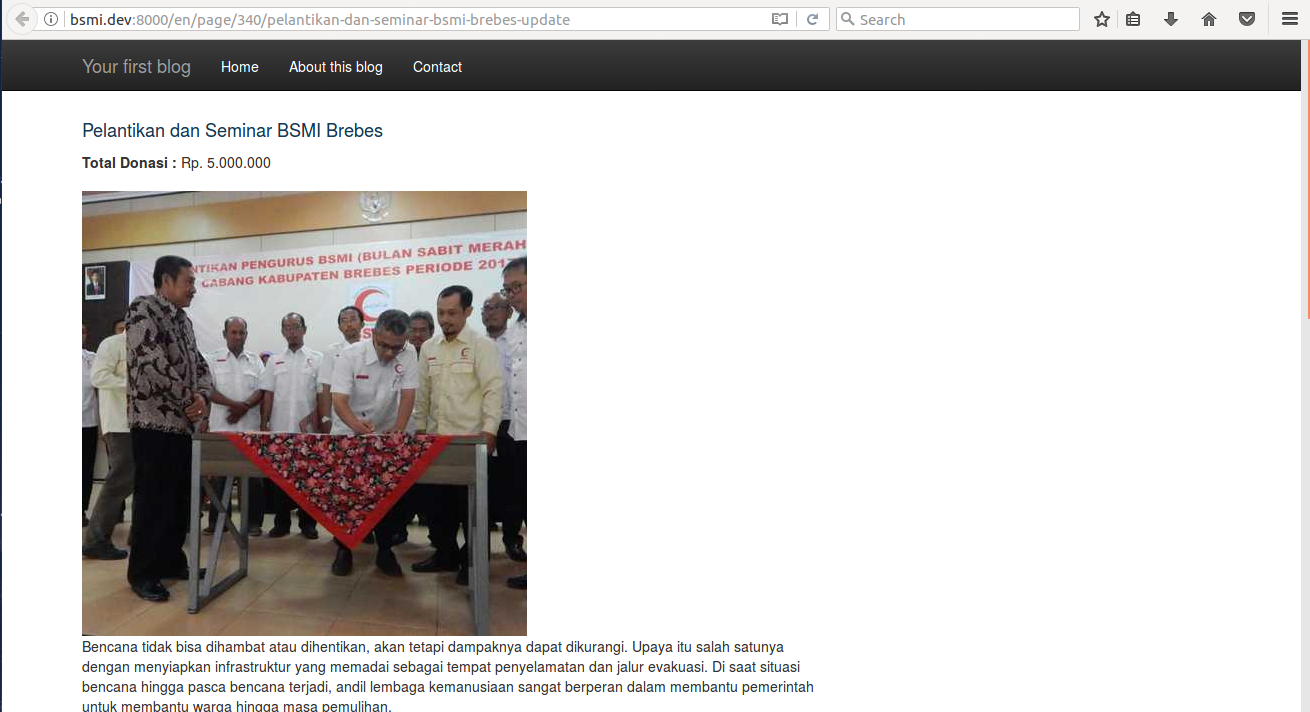
\includegraphics[width=1\textwidth]
	{pics/29-viewprogramupdatedonation.png}
	\caption{Tampilan \textit{page} Pelantikan dan Seminar BSMI Brebes setelah perubahan}
	\label{fig:viewprogram5}
\end{figure}
\vspace{-0.3cm}

\section{Contoh Keterhubungan Data pada Web BSMI}

Setelah pada subbab sebelumnya telah dilakukan proses pembuatan \textit{page} pada web BSMI, pada subbab ini akan membahas mengenai keterhubungan data dari \textit{page-page} yang telah dibuat tersebut. Berbeda dengan \textit{web} pada umumnya, \textit{web} yang menerapkan konsep semantik akan dapat langsung mengolah informasi berdasarkan keterhubungan data yang dimilikinya.

\begin{figure}
	\centering
	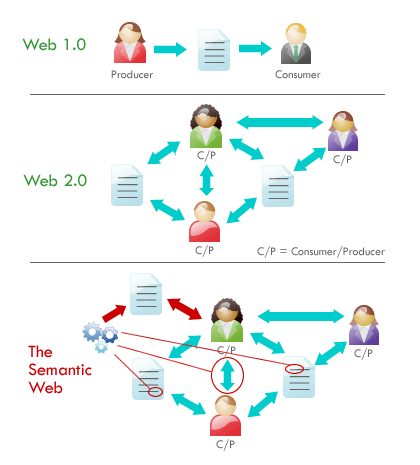
\includegraphics[width=0.5\textwidth]
	{pics/semantic-web.jpg}
	\caption{Perbedaan \textit{web} semantik dengan \textit{web} biasa}
	\label{fig:semanticweb}
\end{figure}
\vspace{-0.3cm}

Pada \pic~\ref{fig:semanticweb}, terdapat perbandingan antara \textit{web} biasa dengan \textit{web} semantik. Pada teknologi \textit{web} 1.0, sebuah \textit{page} khusus dibuat oleh \textit{producer} untuk satu \textit{customer}. Pada teknologi ini, \textit{customer} hanya berperan sebagai pembaca saja. Contohnya dari penerapan teknologi ini adalah blog. Selanjutnya ditemukan teknologi \textit{web} 2.0 dimana \textit{customer} dapat berperan sebagai \textit{producer} juga. Contoh dari penerapan teknologi ini adalah sosial media seperti Twitter, Facebook, dan lain-lain. Namun, pada teknologi ini, informasi-informasi yang ada hanya sebatas untuk ditampilkan saja. Sehingga muncul teknologi \textit{web} 3.0 atau disebut \textit{web} semantik dimana informasi-informasi yang terdapat pada \textit{web} dapat diolah dan ditampilkan pada suatu \textit{page}.

Zotonic sebagai sebuah \textit{web framework} yang telah mengimplementasikan semantik dapat digunakan sebagai sebuah \textit{engine} untuk mengolah dan menampilkan hasilnya pada sebuah \textit{page}. Berikut merupakan hasil dari penerapan keterhubungan data pada \textit{web} BSMI.

\begin{figure}
	\centering
	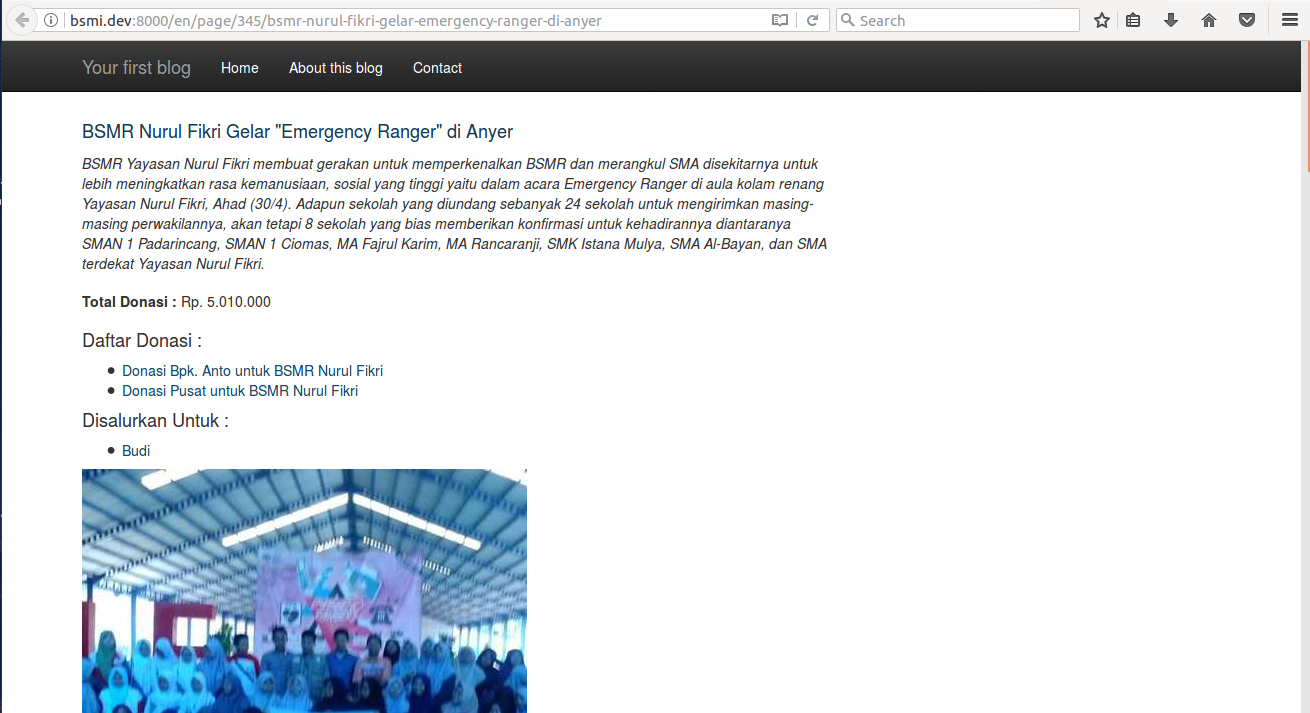
\includegraphics[width=1\textwidth]
	{pics/100-program.png}
	\caption{Tampilan \textit{page Program} yang telah menampilkan keterhubungan data}
	\label{fig:programlinked}
\end{figure}
\vspace{-0.3cm}

Pada \pic~\ref{fig:programlinked}, merupakan tampilan dari sebuah \textit{page} dengan kategori \textit{Program}. Tampilan ini menggabungkan informasi yang didapatkan dari \textit{page} \textit{Target} dan \textit{Donation} untuk ditampilkan pada tampilan \textit{Program}. Pada \textit{page} ini, ditampilkan total donasi yang diterima untuk program ini yang dihitung dari \textit{amount} seluruh donasi yang terhubung ke program ini seperti yang dijelaskan pada bab sebelumnya. Selanjutnya terdapat juga informasi daftar donasi yang diberikan kepada program ini serta informasi disalurkan kepada siapa dana dari program ini.

\begin{figure}
	\centering
	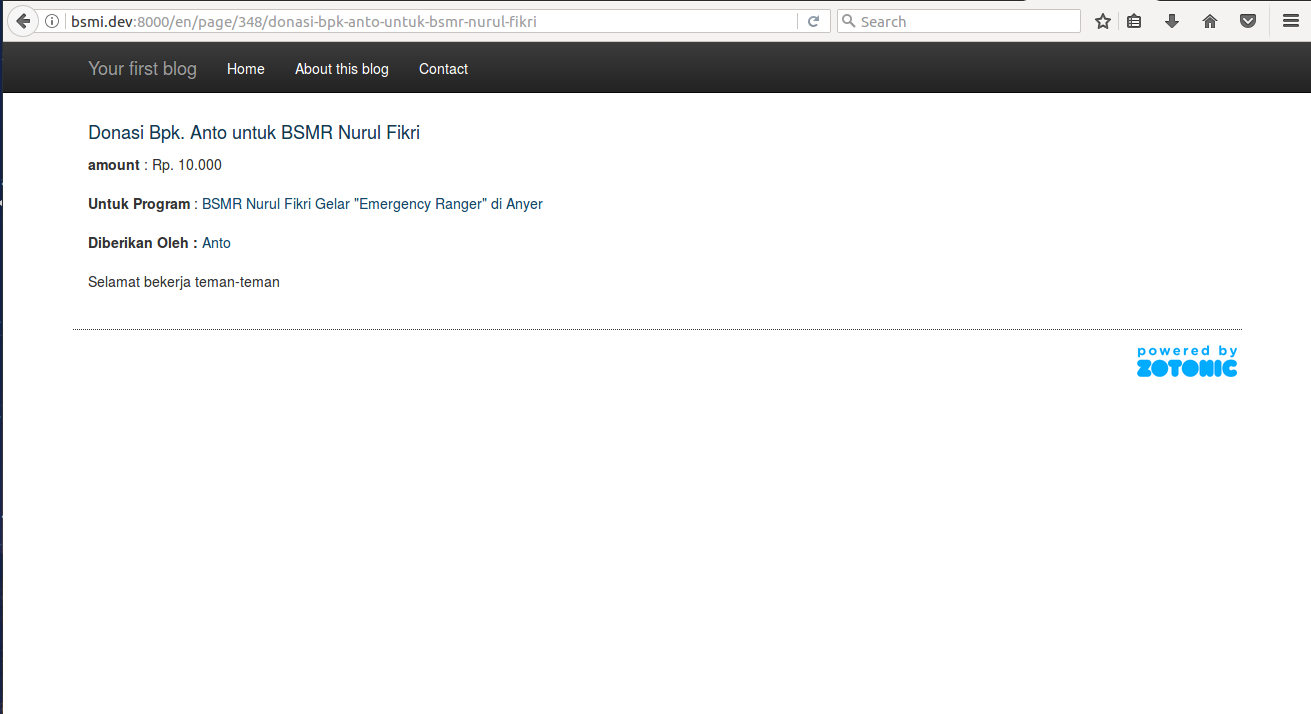
\includegraphics[width=1\textwidth]
	{pics/101-donasi.png}
	\caption{Tampilan \textit{page Donasi} yang telah menampilkan keterhubungan data}
	\label{fig:donationlinked}
\end{figure}
\vspace{-0.3cm}

\begin{figure}
	\centering
	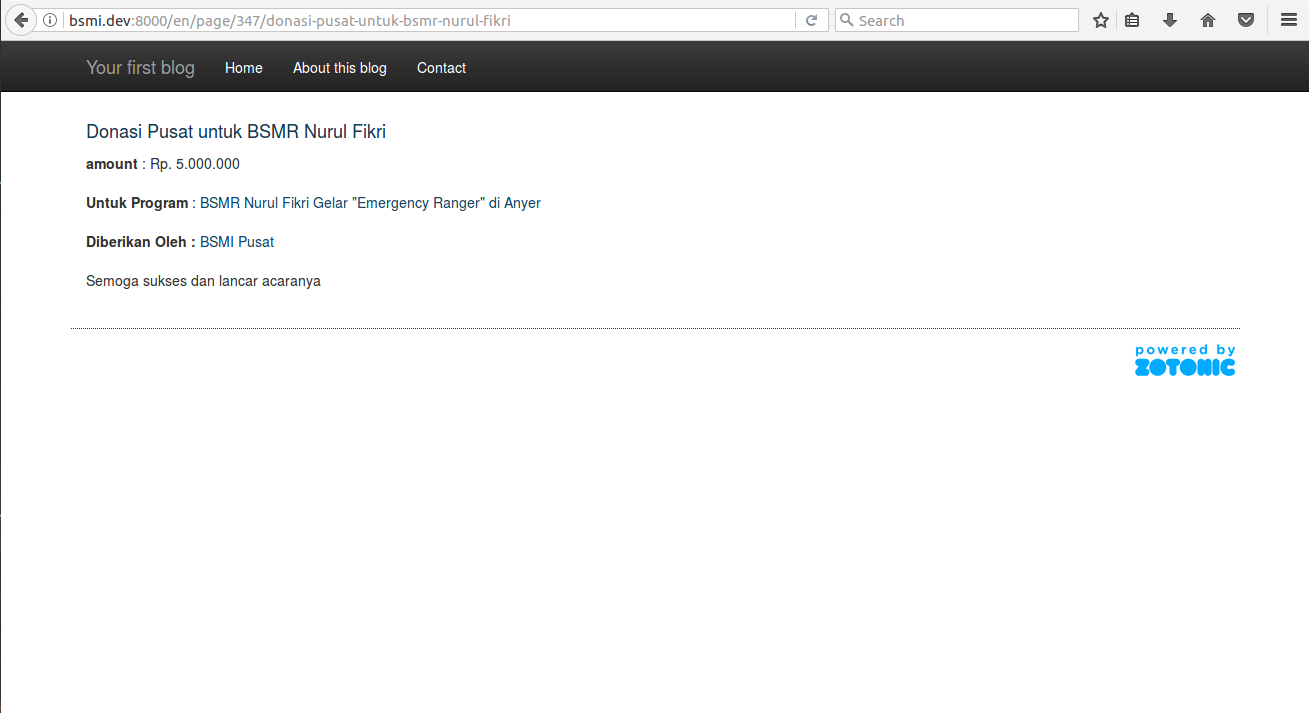
\includegraphics[width=1\textwidth]
	{pics/101-donasi2.png}
	\caption{Tampilan \textit{page Donasi} yang telah menampilkan keterhubungan data}
	\label{fig:donationlinked2}
\end{figure}
\vspace{-0.3cm}

Pada \pic~\ref{fig:donationlinked} dan \pic~\ref{fig:donationlinked2}, merupakan tampilan dari sebuah \textit{page} dengan kategori \textit{Donation}. Tampilan tersebut menggabungkan informasi yang didapatkan dari \textit{page Program} dan \textit{Donor}. Pada \textit{page} tersebut, ditampilkan informasi mengenai donasi tersebut disalurkan untuk program yang mana dan donasi tersebut diberikan oleh siapa.

\section{Kesesuaian Keterhubungan Data dengan Ontologi}

